\documentclass[1p]{elsarticle_modified}
%\bibliographystyle{elsarticle-num}

%\usepackage[colorlinks]{hyperref}
%\usepackage{abbrmath_seonhwa} %\Abb, \Ascr, \Acal ,\Abf, \Afrak
\usepackage{amsfonts}
\usepackage{amssymb}
\usepackage{amsmath}
\usepackage{amsthm}
\usepackage{scalefnt}
\usepackage{amsbsy}
\usepackage{kotex}
\usepackage{caption}
\usepackage{subfig}
\usepackage{color}
\usepackage{graphicx}
\usepackage{xcolor} %% white, black, red, green, blue, cyan, magenta, yellow
\usepackage{float}
\usepackage{setspace}
\usepackage{hyperref}

\usepackage{tikz}
\usetikzlibrary{arrows}

\usepackage{multirow}
\usepackage{array} % fixed length table
\usepackage{hhline}

%%%%%%%%%%%%%%%%%%%%%
\makeatletter
\renewcommand*\env@matrix[1][\arraystretch]{%
	\edef\arraystretch{#1}%
	\hskip -\arraycolsep
	\let\@ifnextchar\new@ifnextchar
	\array{*\c@MaxMatrixCols c}}
\makeatother %https://tex.stackexchange.com/questions/14071/how-can-i-increase-the-line-spacing-in-a-matrix
%%%%%%%%%%%%%%%

\usepackage[normalem]{ulem}

\newcommand{\msout}[1]{\ifmmode\text{\sout{\ensuremath{#1}}}\else\sout{#1}\fi}
%SOURCE: \msout is \stkout macro in https://tex.stackexchange.com/questions/20609/strikeout-in-math-mode

\newcommand{\cancel}[1]{
	\ifmmode
	{\color{red}\msout{#1}}
	\else
	{\color{red}\sout{#1}}
	\fi
}

\newcommand{\add}[1]{
	{\color{blue}\uwave{#1}}
}

\newcommand{\replace}[2]{
	\ifmmode
	{\color{red}\msout{#1}}{\color{blue}\uwave{#2}}
	\else
	{\color{red}\sout{#1}}{\color{blue}\uwave{#2}}
	\fi
}

\newcommand{\Sol}{\mathcal{S}} %segment
\newcommand{\D}{D} %diagram
\newcommand{\A}{\mathcal{A}} %arc


%%%%%%%%%%%%%%%%%%%%%%%%%%%%%5 test

\def\sl{\operatorname{\textup{SL}}(2,\Cbb)}
\def\psl{\operatorname{\textup{PSL}}(2,\Cbb)}
\def\quan{\mkern 1mu \triangleright \mkern 1mu}

\theoremstyle{definition}
\newtheorem{thm}{Theorem}[section]
\newtheorem{prop}[thm]{Proposition}
\newtheorem{lem}[thm]{Lemma}
\newtheorem{ques}[thm]{Question}
\newtheorem{cor}[thm]{Corollary}
\newtheorem{defn}[thm]{Definition}
\newtheorem{exam}[thm]{Example}
\newtheorem{rmk}[thm]{Remark}
\newtheorem{alg}[thm]{Algorithm}

\newcommand{\I}{\sqrt{-1}}
\begin{document}

%\begin{frontmatter}
%
%\title{Boundary parabolic representations of knots up to 8 crossings}
%
%%% Group authors per affiliation:
%\author{Yunhi Cho} 
%\address{Department of Mathematics, University of Seoul, Seoul, Korea}
%\ead{yhcho@uos.ac.kr}
%
%
%\author{Seonhwa Kim} %\fnref{s_kim}}
%\address{Center for Geometry and Physics, Institute for Basic Science, Pohang, 37673, Korea}
%\ead{ryeona17@ibs.re.kr}
%
%\author{Hyuk Kim}
%\address{Department of Mathematical Sciences, Seoul National University, Seoul 08826, Korea}
%\ead{hyukkim@snu.ac.kr}
%
%\author{Seokbeom Yoon}
%\address{Department of Mathematical Sciences, Seoul National University, Seoul, 08826,  Korea}
%\ead{sbyoon15@snu.ac.kr}
%
%\begin{abstract}
%We find all boundary parabolic representation of knots up to 8 crossings.
%
%\end{abstract}
%\begin{keyword}
%    \MSC[2010] 57M25 
%\end{keyword}
%
%\end{frontmatter}

%\linenumbers
%\tableofcontents
%
\newcommand\colored[1]{\textcolor{white}{\rule[-0.35ex]{0.8em}{1.4ex}}\kern-0.8em\color{red} #1}%
%\newcommand\colored[1]{\textcolor{white}{ #1}\kern-2.17ex	\textcolor{white}{ #1}\kern-1.81ex	\textcolor{white}{ #1}\kern-2.15ex\color{red}#1	}

{\Large $\underline{12a_{1188}~(K12a_{1188})}$}

\setlength{\tabcolsep}{10pt}
\renewcommand{\arraystretch}{1.6}
\vspace{1cm}\begin{tabular}{m{100pt}>{\centering\arraybackslash}m{274pt}}
\multirow{5}{120pt}{
	\centering
	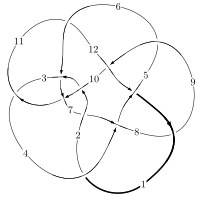
\includegraphics[width=112pt]{../../../GIT/diagram.site/Diagrams/png/1989_12a_1188.png}\\
\ \ \ A knot diagram\footnotemark}&
\allowdisplaybreaks
\textbf{Linearized knot diagam} \\
\cline{2-2}
 &
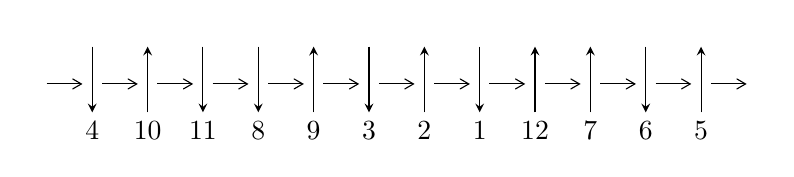
\begin{tikzpicture}[x=20pt, y=17pt]
	% nodes
	\node (C0) at (0, 0) {};
	\node (C1) at (1, 0) {};
	\node (C1U) at (1, +1) {};
	\node (C1D) at (1, -1) {4};

	\node (C2) at (2, 0) {};
	\node (C2U) at (2, +1) {};
	\node (C2D) at (2, -1) {10};

	\node (C3) at (3, 0) {};
	\node (C3U) at (3, +1) {};
	\node (C3D) at (3, -1) {11};

	\node (C4) at (4, 0) {};
	\node (C4U) at (4, +1) {};
	\node (C4D) at (4, -1) {8};

	\node (C5) at (5, 0) {};
	\node (C5U) at (5, +1) {};
	\node (C5D) at (5, -1) {9};

	\node (C6) at (6, 0) {};
	\node (C6U) at (6, +1) {};
	\node (C6D) at (6, -1) {3};

	\node (C7) at (7, 0) {};
	\node (C7U) at (7, +1) {};
	\node (C7D) at (7, -1) {2};

	\node (C8) at (8, 0) {};
	\node (C8U) at (8, +1) {};
	\node (C8D) at (8, -1) {1};

	\node (C9) at (9, 0) {};
	\node (C9U) at (9, +1) {};
	\node (C9D) at (9, -1) {12};

	\node (C10) at (10, 0) {};
	\node (C10U) at (10, +1) {};
	\node (C10D) at (10, -1) {7};

	\node (C11) at (11, 0) {};
	\node (C11U) at (11, +1) {};
	\node (C11D) at (11, -1) {6};

	\node (C12) at (12, 0) {};
	\node (C12U) at (12, +1) {};
	\node (C12D) at (12, -1) {5};
	\node (C13) at (13, 0) {};

	% arrows
	\draw[->,>={angle 60}]
	(C0) edge (C1) (C1) edge (C2) (C2) edge (C3) (C3) edge (C4) (C4) edge (C5) (C5) edge (C6) (C6) edge (C7) (C7) edge (C8) (C8) edge (C9) (C9) edge (C10) (C10) edge (C11) (C11) edge (C12) (C12) edge (C13) ;	\draw[->,>=stealth]
	(C1U) edge (C1D) (C2D) edge (C2U) (C3U) edge (C3D) (C4U) edge (C4D) (C5D) edge (C5U) (C6U) edge (C6D) (C7D) edge (C7U) (C8U) edge (C8D) (C9D) edge (C9U) (C10D) edge (C10U) (C11U) edge (C11D) (C12D) edge (C12U) ;
	\end{tikzpicture} \\
\hhline{~~} \\& 
\textbf{Solving Sequence} \\ \cline{2-2} 
 &
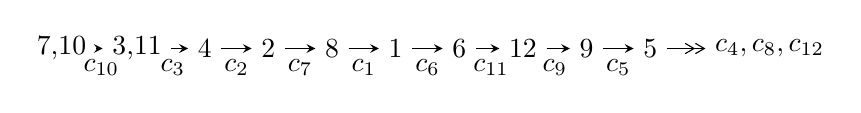
\begin{tikzpicture}[x=23pt, y=7pt]
	% node
	\node (A0) at (-1/8, 0) {7,10};
	\node (A1) at (17/16, 0) {3,11};
	\node (A2) at (17/8, 0) {4};
	\node (A3) at (25/8, 0) {2};
	\node (A4) at (33/8, 0) {8};
	\node (A5) at (41/8, 0) {1};
	\node (A6) at (49/8, 0) {6};
	\node (A7) at (57/8, 0) {12};
	\node (A8) at (65/8, 0) {9};
	\node (A9) at (73/8, 0) {5};
	\node (C1) at (1/2, -1) {$c_{10}$};
	\node (C2) at (13/8, -1) {$c_{3}$};
	\node (C3) at (21/8, -1) {$c_{2}$};
	\node (C4) at (29/8, -1) {$c_{7}$};
	\node (C5) at (37/8, -1) {$c_{1}$};
	\node (C6) at (45/8, -1) {$c_{6}$};
	\node (C7) at (53/8, -1) {$c_{11}$};
	\node (C8) at (61/8, -1) {$c_{9}$};
	\node (C9) at (69/8, -1) {$c_{5}$};
	\node (A10) at (11, 0) {$c_{4},c_{8},c_{12}$};

	% edge
	\draw[->,>=stealth]	
	(A0) edge (A1) (A1) edge (A2) (A2) edge (A3) (A3) edge (A4) (A4) edge (A5) (A5) edge (A6) (A6) edge (A7) (A7) edge (A8) (A8) edge (A9) ;
	\draw[->>,>={angle 60}]	
	(A9) edge (A10);
\end{tikzpicture} \\ 

\end{tabular} \\

\footnotetext{
The image of knot diagram is generated by the software ``\textbf{Draw programme}" developed by Andrew Bartholomew(\url{http://www.layer8.co.uk/maths/draw/index.htm\#Running-draw}), where we modified some parts for our purpose(\url{https://github.com/CATsTAILs/LinksPainter}).
}\phantom \\ \newline 
\centering \textbf{Ideals for irreducible components\footnotemark of $X_{\text{par}}$} 
 
\begin{align*}
I^u_{1}&=\langle 
1.81506\times10^{2919} u^{239}-1.08972\times10^{2920} u^{238}+\cdots+4.30429\times10^{2919} b-1.97379\times10^{2919},\\
\phantom{I^u_{1}}&\phantom{= \langle  }-5.27544\times10^{2905} u^{239}+3.16294\times10^{2906} u^{238}+\cdots+1.89211\times10^{2905} a+1.16747\times10^{2906},\\
\phantom{I^u_{1}}&\phantom{= \langle  }u^{240}-6 u^{239}+\cdots+10 u+1\rangle \\
I^u_{2}&=\langle 
-2.64041\times10^{167} u^{63}+8.31490\times10^{167} u^{62}+\cdots+4.36412\times10^{167} b+2.46869\times10^{167},\\
\phantom{I^u_{2}}&\phantom{= \langle  }8.16860\times10^{164} u^{63}-2.18885\times10^{165} u^{62}+\cdots+1.84218\times10^{164} a-3.02215\times10^{164},\;u^{64}-3 u^{63}+\cdots-2 u+1\rangle \\
\\
\end{align*}
\raggedright * 2 irreducible components of $\dim_{\mathbb{C}}=0$, with total 304 representations.\\
\footnotetext{All coefficients of polynomials are rational numbers. But the coefficients are sometimes approximated in decimal forms when there is not enough margin.}
\newpage
\renewcommand{\arraystretch}{1}
\centering \section*{I. $I^u_{1}= \langle 1.82\times10^{2919} u^{239}-1.09\times10^{2920} u^{238}+\cdots+4.30\times10^{2919} b-1.97\times10^{2919},\;-5.28\times10^{2905} u^{239}+3.16\times10^{2906} u^{238}+\cdots+1.89\times10^{2905} a+1.17\times10^{2906},\;u^{240}-6 u^{239}+\cdots+10 u+1 \rangle$}
\flushleft \textbf{(i) Arc colorings}\\
\begin{tabular}{m{7pt} m{180pt} m{7pt} m{180pt} }
\flushright $a_{7}=$&$\begin{pmatrix}0\\u\end{pmatrix}$ \\
\flushright $a_{10}=$&$\begin{pmatrix}1\\0\end{pmatrix}$ \\
\flushright $a_{3}=$&$\begin{pmatrix}2.78813 u^{239}-16.7165 u^{238}+\cdots-5.43938 u-6.17024\\-0.421687 u^{239}+2.53172 u^{238}+\cdots+6.21740 u+0.458564\end{pmatrix}$ \\
\flushright $a_{11}=$&$\begin{pmatrix}1\\- u^2\end{pmatrix}$ \\
\flushright $a_{4}=$&$\begin{pmatrix}3.25402 u^{239}-19.5063 u^{238}+\cdots-8.74602 u-6.61654\\-0.384909 u^{239}+2.30152 u^{238}+\cdots+6.73880 u+0.464116\end{pmatrix}$ \\
\flushright $a_{2}=$&$\begin{pmatrix}3.20982 u^{239}-19.2483 u^{238}+\cdots-11.6568 u-6.62880\\-0.421687 u^{239}+2.53172 u^{238}+\cdots+6.21740 u+0.458564\end{pmatrix}$ \\
\flushright $a_{8}=$&$\begin{pmatrix}3.66418 u^{239}-21.6821 u^{238}+\cdots+143.995 u-9.87242\\-0.0549898 u^{239}+0.268874 u^{238}+\cdots+15.4207 u+3.35693\end{pmatrix}$ \\
\flushright $a_{1}=$&$\begin{pmatrix}3.81437 u^{239}-22.9434 u^{238}+\cdots+2.58637 u-6.43776\\-0.446474 u^{239}+2.66940 u^{238}+\cdots+6.43698 u-0.125884\end{pmatrix}$ \\
\flushright $a_{6}=$&$\begin{pmatrix}3.56736 u^{239}-21.2165 u^{238}+\cdots+171.565 u-3.31915\\-0.0418322 u^{239}+0.196767 u^{238}+\cdots+14.1492 u+3.19633\end{pmatrix}$ \\
\flushright $a_{12}=$&$\begin{pmatrix}1.50713 u^{239}-9.09463 u^{238}+\cdots+30.2331 u-0.181601\\0.112580 u^{239}-0.719524 u^{238}+\cdots+2.39539 u+0.954201\end{pmatrix}$ \\
\flushright $a_{9}=$&$\begin{pmatrix}1.04405 u^{239}-6.46589 u^{238}+\cdots-32.4340 u-4.21920\\-0.615053 u^{239}+3.78553 u^{238}+\cdots-6.21318 u-1.93610\end{pmatrix}$ \\
\flushright $a_{5}=$&$\begin{pmatrix}6.38370 u^{239}-38.1804 u^{238}+\cdots+325.441 u+6.54059\\-0.817778 u^{239}+4.98347 u^{238}+\cdots-8.13549 u-0.697420\end{pmatrix}$\\&\end{tabular}
\flushleft \textbf{(ii) Obstruction class $= -1$}\\~\\
\flushleft \textbf{(iii) Cusp Shapes $= 1.57847 u^{239}-10.3573 u^{238}+\cdots-181.846 u-1.67149$}\\~\\
\newpage\renewcommand{\arraystretch}{1}
\flushleft \textbf{(iv) u-Polynomials at the component}\newline \\
\begin{tabular}{m{50pt}|m{274pt}}
Crossings & \hspace{64pt}u-Polynomials at each crossing \\
\hline $$\begin{aligned}c_{1}\end{aligned}$$&$\begin{aligned}
&u^{240}+11 u^{239}+\cdots-149360 u+19984
\end{aligned}$\\
\hline $$\begin{aligned}c_{2}\end{aligned}$$&$\begin{aligned}
&u^{240}+u^{239}+\cdots+81 u+1
\end{aligned}$\\
\hline $$\begin{aligned}c_{3}\end{aligned}$$&$\begin{aligned}
&u^{240}- u^{239}+\cdots-81 u+1
\end{aligned}$\\
\hline $$\begin{aligned}c_{4}\end{aligned}$$&$\begin{aligned}
&u^{240}+3 u^{239}+\cdots+2694745 u+109393
\end{aligned}$\\
\hline $$\begin{aligned}c_{5}\end{aligned}$$&$\begin{aligned}
&u^{240}-3 u^{239}+\cdots-2694745 u+109393
\end{aligned}$\\
\hline $$\begin{aligned}c_{6}\end{aligned}$$&$\begin{aligned}
&u^{240}+6 u^{239}+\cdots-10 u+1
\end{aligned}$\\
\hline $$\begin{aligned}c_{7}\end{aligned}$$&$\begin{aligned}
&u^{240}+u^{239}+\cdots+412134229504 u+89704305664
\end{aligned}$\\
\hline $$\begin{aligned}c_{8}\end{aligned}$$&$\begin{aligned}
&u^{240}+17 u^{238}+\cdots-455354 u+53269
\end{aligned}$\\
\hline $$\begin{aligned}c_{9}\end{aligned}$$&$\begin{aligned}
&u^{240}-11 u^{239}+\cdots+149360 u+19984
\end{aligned}$\\
\hline $$\begin{aligned}c_{10}\end{aligned}$$&$\begin{aligned}
&u^{240}-6 u^{239}+\cdots+10 u+1
\end{aligned}$\\
\hline $$\begin{aligned}c_{11}\end{aligned}$$&$\begin{aligned}
&u^{240}- u^{239}+\cdots-412134229504 u+89704305664
\end{aligned}$\\
\hline $$\begin{aligned}c_{12}\end{aligned}$$&$\begin{aligned}
&u^{240}+17 u^{238}+\cdots+455354 u+53269
\end{aligned}$\\
\hline
\end{tabular}\\~\\
\newpage\renewcommand{\arraystretch}{1}
\flushleft \textbf{(v) Riley Polynomials at the component}\newline \\
\begin{tabular}{m{50pt}|m{274pt}}
Crossings & \hspace{64pt}Riley Polynomials at each crossing \\
\hline $$\begin{aligned}c_{1},c_{9}\end{aligned}$$&$\begin{aligned}
&y^{240}+19 y^{239}+\cdots+58000092160 y+399360256
\end{aligned}$\\
\hline $$\begin{aligned}c_{2},c_{3}\end{aligned}$$&$\begin{aligned}
&y^{240}+31 y^{239}+\cdots-443 y+1
\end{aligned}$\\
\hline $$\begin{aligned}c_{4},c_{5}\end{aligned}$$&$\begin{aligned}
&y^{240}-31 y^{239}+\cdots-2123917792621 y+11966828449
\end{aligned}$\\
\hline $$\begin{aligned}c_{6},c_{10}\end{aligned}$$&$\begin{aligned}
&y^{240}+24 y^{239}+\cdots+176 y+1
\end{aligned}$\\
\hline $$\begin{aligned}c_{7},c_{11}\end{aligned}$$&$\begin{aligned}
&y^{240}+79 y^{239}+\cdots-5.06\times10^{23} y+8.05\times10^{21}
\end{aligned}$\\
\hline $$\begin{aligned}c_{8},c_{12}\end{aligned}$$&$\begin{aligned}
&y^{240}+34 y^{239}+\cdots+461228757544 y+2837586361
\end{aligned}$\\
\hline
\end{tabular}\\~\\
\newpage\flushleft \textbf{(vi) Complex Volumes and Cusp Shapes}
$$\begin{array}{c|c|c}  
\text{Solutions to }I^u_{1}& \I (\text{vol} + \sqrt{-1}CS) & \text{Cusp shape}\\
 \hline 
\begin{aligned}
u &= -0.462173 + 0.889612 I \\
a &= -1.205520 - 0.585035 I \\
b &= -0.130224 - 0.650718 I\end{aligned}
 & -1.66054 + 0.42784 I & \phantom{-0.000000 } 0 \\ \hline\begin{aligned}
u &= -0.462173 - 0.889612 I \\
a &= -1.205520 + 0.585035 I \\
b &= -0.130224 + 0.650718 I\end{aligned}
 & -1.66054 - 0.42784 I & \phantom{-0.000000 } 0 \\ \hline\begin{aligned}
u &= -0.955315 + 0.283983 I \\
a &= -0.265351 + 0.329439 I \\
b &= -1.04054 + 1.12378 I\end{aligned}
 & \phantom{-}2.32347 - 4.18248 I & \phantom{-0.000000 } 0 \\ \hline\begin{aligned}
u &= -0.955315 - 0.283983 I \\
a &= -0.265351 - 0.329439 I \\
b &= -1.04054 - 1.12378 I\end{aligned}
 & \phantom{-}2.32347 + 4.18248 I & \phantom{-0.000000 } 0 \\ \hline\begin{aligned}
u &= -0.752413 + 0.653296 I \\
a &= \phantom{-}0.594249 - 0.646863 I \\
b &= -0.355511 + 0.287540 I\end{aligned}
 & -1.83854 - 2.39098 I & \phantom{-0.000000 } 0 \\ \hline\begin{aligned}
u &= -0.752413 - 0.653296 I \\
a &= \phantom{-}0.594249 + 0.646863 I \\
b &= -0.355511 - 0.287540 I\end{aligned}
 & -1.83854 + 2.39098 I & \phantom{-0.000000 } 0 \\ \hline\begin{aligned}
u &= -0.564784 + 0.843184 I \\
a &= -0.25618 + 1.62455 I \\
b &= -0.94983 + 1.54327 I\end{aligned}
 & \phantom{-}1.95547 - 5.70601 I & \phantom{-0.000000 } 0 \\ \hline\begin{aligned}
u &= -0.564784 - 0.843184 I \\
a &= -0.25618 - 1.62455 I \\
b &= -0.94983 - 1.54327 I\end{aligned}
 & \phantom{-}1.95547 + 5.70601 I & \phantom{-0.000000 } 0 \\ \hline\begin{aligned}
u &= -0.112788 + 0.974457 I \\
a &= -1.33083 + 0.78769 I \\
b &= -0.160752 + 0.511728 I\end{aligned}
 & -3.13991 - 10.22530 I & \phantom{-0.000000 } 0 \\ \hline\begin{aligned}
u &= -0.112788 - 0.974457 I \\
a &= -1.33083 - 0.78769 I \\
b &= -0.160752 - 0.511728 I\end{aligned}
 & -3.13991 + 10.22530 I & \phantom{-0.000000 } 0\\
 \hline 
 \end{array}$$\newpage$$\begin{array}{c|c|c}  
\text{Solutions to }I^u_{1}& \I (\text{vol} + \sqrt{-1}CS) & \text{Cusp shape}\\
 \hline 
\begin{aligned}
u &= \phantom{-}0.851605 + 0.574305 I \\
a &= \phantom{-}0.117778 + 0.090949 I \\
b &= \phantom{-}0.916781 + 0.207243 I\end{aligned}
 & \phantom{-}0.95651 + 1.30346 I & \phantom{-0.000000 } 0 \\ \hline\begin{aligned}
u &= \phantom{-}0.851605 - 0.574305 I \\
a &= \phantom{-}0.117778 - 0.090949 I \\
b &= \phantom{-}0.916781 - 0.207243 I\end{aligned}
 & \phantom{-}0.95651 - 1.30346 I & \phantom{-0.000000 } 0 \\ \hline\begin{aligned}
u &= \phantom{-}0.962888 + 0.076989 I \\
a &= -0.123291 - 0.677784 I \\
b &= -0.61778 - 1.59419 I\end{aligned}
 & \phantom{-}3.77428 + 3.63498 I & \phantom{-0.000000 } 0 \\ \hline\begin{aligned}
u &= \phantom{-}0.962888 - 0.076989 I \\
a &= -0.123291 + 0.677784 I \\
b &= -0.61778 + 1.59419 I\end{aligned}
 & \phantom{-}3.77428 - 3.63498 I & \phantom{-0.000000 } 0 \\ \hline\begin{aligned}
u &= -0.758729 + 0.593105 I \\
a &= -0.04017 + 1.56316 I \\
b &= -0.861363 + 0.697584 I\end{aligned}
 & \phantom{-}6.08093 - 2.08294 I & \phantom{-0.000000 } 0 \\ \hline\begin{aligned}
u &= -0.758729 - 0.593105 I \\
a &= -0.04017 - 1.56316 I \\
b &= -0.861363 - 0.697584 I\end{aligned}
 & \phantom{-}6.08093 + 2.08294 I & \phantom{-0.000000 } 0 \\ \hline\begin{aligned}
u &= -1.027460 + 0.144503 I \\
a &= \phantom{-}0.961208 + 0.275825 I \\
b &= -0.538282 + 0.432730 I\end{aligned}
 & \phantom{-0.000000 } -6.17244 I & \phantom{-0.000000 } 0 \\ \hline\begin{aligned}
u &= -1.027460 - 0.144503 I \\
a &= \phantom{-}0.961208 - 0.275825 I \\
b &= -0.538282 - 0.432730 I\end{aligned}
 & \phantom{-0.000000 -}6.17244 I & \phantom{-0.000000 } 0 \\ \hline\begin{aligned}
u &= \phantom{-}0.983829 + 0.361988 I \\
a &= -0.162275 + 0.616807 I \\
b &= -0.249772 + 1.272020 I\end{aligned}
 & \phantom{-}3.26283 + 2.70754 I & \phantom{-0.000000 } 0 \\ \hline\begin{aligned}
u &= \phantom{-}0.983829 - 0.361988 I \\
a &= -0.162275 - 0.616807 I \\
b &= -0.249772 - 1.272020 I\end{aligned}
 & \phantom{-}3.26283 - 2.70754 I & \phantom{-0.000000 } 0\\
 \hline 
 \end{array}$$\newpage$$\begin{array}{c|c|c}  
\text{Solutions to }I^u_{1}& \I (\text{vol} + \sqrt{-1}CS) & \text{Cusp shape}\\
 \hline 
\begin{aligned}
u &= -0.843979 + 0.626338 I \\
a &= \phantom{-}0.11343 + 1.56019 I \\
b &= -0.775740 + 0.550166 I\end{aligned}
 & \phantom{-}5.39279 - 6.94228 I & \phantom{-0.000000 } 0 \\ \hline\begin{aligned}
u &= -0.843979 - 0.626338 I \\
a &= \phantom{-}0.11343 - 1.56019 I \\
b &= -0.775740 - 0.550166 I\end{aligned}
 & \phantom{-}5.39279 + 6.94228 I & \phantom{-0.000000 } 0 \\ \hline\begin{aligned}
u &= -0.172009 + 1.038400 I \\
a &= \phantom{-}0.519630 - 1.309040 I \\
b &= \phantom{-}0.146076 - 0.681818 I\end{aligned}
 & -2.54684 - 2.74438 I & \phantom{-0.000000 } 0 \\ \hline\begin{aligned}
u &= -0.172009 - 1.038400 I \\
a &= \phantom{-}0.519630 + 1.309040 I \\
b &= \phantom{-}0.146076 + 0.681818 I\end{aligned}
 & -2.54684 + 2.74438 I & \phantom{-0.000000 } 0 \\ \hline\begin{aligned}
u &= \phantom{-}0.732181 + 0.588336 I \\
a &= -0.190030 + 0.674014 I \\
b &= \phantom{-}0.795753 + 0.513770 I\end{aligned}
 & \phantom{-}1.36746 + 1.23188 I & \phantom{-0.000000 } 0 \\ \hline\begin{aligned}
u &= \phantom{-}0.732181 - 0.588336 I \\
a &= -0.190030 - 0.674014 I \\
b &= \phantom{-}0.795753 - 0.513770 I\end{aligned}
 & \phantom{-}1.36746 - 1.23188 I & \phantom{-0.000000 } 0 \\ \hline\begin{aligned}
u &= \phantom{-}0.621211 + 0.869444 I \\
a &= -0.47955 - 1.65018 I \\
b &= -1.21639 - 0.92379 I\end{aligned}
 & \phantom{-}2.94911 + 3.94406 I & \phantom{-0.000000 } 0 \\ \hline\begin{aligned}
u &= \phantom{-}0.621211 - 0.869444 I \\
a &= -0.47955 + 1.65018 I \\
b &= -1.21639 + 0.92379 I\end{aligned}
 & \phantom{-}2.94911 - 3.94406 I & \phantom{-0.000000 } 0 \\ \hline\begin{aligned}
u &= \phantom{-}0.254211 + 1.039930 I \\
a &= \phantom{-}0.300450 - 0.075517 I \\
b &= \phantom{-}1.48858 - 0.42954 I\end{aligned}
 & -1.50146 + 0.64615 I & \phantom{-0.000000 } 0 \\ \hline\begin{aligned}
u &= \phantom{-}0.254211 - 1.039930 I \\
a &= \phantom{-}0.300450 + 0.075517 I \\
b &= \phantom{-}1.48858 + 0.42954 I\end{aligned}
 & -1.50146 - 0.64615 I & \phantom{-0.000000 } 0\\
 \hline 
 \end{array}$$\newpage$$\begin{array}{c|c|c}  
\text{Solutions to }I^u_{1}& \I (\text{vol} + \sqrt{-1}CS) & \text{Cusp shape}\\
 \hline 
\begin{aligned}
u &= -0.873327 + 0.627565 I \\
a &= \phantom{-}0.07075 - 1.45313 I \\
b &= \phantom{-}1.111060 - 0.393869 I\end{aligned}
 & \phantom{-}5.34578 + 4.51566 I & \phantom{-0.000000 } 0 \\ \hline\begin{aligned}
u &= -0.873327 - 0.627565 I \\
a &= \phantom{-}0.07075 + 1.45313 I \\
b &= \phantom{-}1.111060 + 0.393869 I\end{aligned}
 & \phantom{-}5.34578 - 4.51566 I & \phantom{-0.000000 } 0 \\ \hline\begin{aligned}
u &= \phantom{-}0.974649 + 0.487952 I \\
a &= \phantom{-}0.100632 - 1.083240 I \\
b &= -0.53954 - 1.51937 I\end{aligned}
 & \phantom{-}1.60477 + 7.07465 I & \phantom{-0.000000 } 0 \\ \hline\begin{aligned}
u &= \phantom{-}0.974649 - 0.487952 I \\
a &= \phantom{-}0.100632 + 1.083240 I \\
b &= -0.53954 + 1.51937 I\end{aligned}
 & \phantom{-}1.60477 - 7.07465 I & \phantom{-0.000000 } 0 \\ \hline\begin{aligned}
u &= -0.307093 + 0.851024 I \\
a &= \phantom{-}0.578632 - 1.127990 I \\
b &= -0.178633 - 0.580618 I\end{aligned}
 & -1.87666 - 1.61146 I & \phantom{-0.000000 } 0 \\ \hline\begin{aligned}
u &= -0.307093 - 0.851024 I \\
a &= \phantom{-}0.578632 + 1.127990 I \\
b &= -0.178633 + 0.580618 I\end{aligned}
 & -1.87666 + 1.61146 I & \phantom{-0.000000 } 0 \\ \hline\begin{aligned}
u &= \phantom{-}0.511715 + 0.737443 I \\
a &= -0.710951 + 0.653603 I \\
b &= \phantom{-}0.523693 + 0.557440 I\end{aligned}
 & \phantom{-}1.43357 + 1.49420 I & \phantom{-0.000000 } 0 \\ \hline\begin{aligned}
u &= \phantom{-}0.511715 - 0.737443 I \\
a &= -0.710951 - 0.653603 I \\
b &= \phantom{-}0.523693 - 0.557440 I\end{aligned}
 & \phantom{-}1.43357 - 1.49420 I & \phantom{-0.000000 } 0 \\ \hline\begin{aligned}
u &= \phantom{-}0.672934 + 0.875350 I \\
a &= -0.0671478 - 0.0909015 I \\
b &= -0.300114 + 0.615676 I\end{aligned}
 & -0.31028 + 2.82362 I & \phantom{-0.000000 } 0 \\ \hline\begin{aligned}
u &= \phantom{-}0.672934 - 0.875350 I \\
a &= -0.0671478 + 0.0909015 I \\
b &= -0.300114 - 0.615676 I\end{aligned}
 & -0.31028 - 2.82362 I & \phantom{-0.000000 } 0\\
 \hline 
 \end{array}$$\newpage$$\begin{array}{c|c|c}  
\text{Solutions to }I^u_{1}& \I (\text{vol} + \sqrt{-1}CS) & \text{Cusp shape}\\
 \hline 
\begin{aligned}
u &= -1.082270 + 0.254160 I \\
a &= \phantom{-}0.160105 - 0.746243 I \\
b &= \phantom{-}0.058687 - 0.807551 I\end{aligned}
 & \phantom{-}3.77157 - 4.59426 I & \phantom{-0.000000 } 0 \\ \hline\begin{aligned}
u &= -1.082270 - 0.254160 I \\
a &= \phantom{-}0.160105 + 0.746243 I \\
b &= \phantom{-}0.058687 + 0.807551 I\end{aligned}
 & \phantom{-}3.77157 + 4.59426 I & \phantom{-0.000000 } 0 \\ \hline\begin{aligned}
u &= -0.024528 + 0.874929 I \\
a &= \phantom{-}0.770188 + 0.838379 I \\
b &= \phantom{-}0.908644 + 0.386792 I\end{aligned}
 & \phantom{-}1.83854 + 2.39098 I & \phantom{-0.000000 } 0 \\ \hline\begin{aligned}
u &= -0.024528 - 0.874929 I \\
a &= \phantom{-}0.770188 - 0.838379 I \\
b &= \phantom{-}0.908644 - 0.386792 I\end{aligned}
 & \phantom{-}1.83854 - 2.39098 I & \phantom{-0.000000 } 0 \\ \hline\begin{aligned}
u &= -0.845800 + 0.189828 I \\
a &= -0.762292 + 0.700803 I \\
b &= -0.230871 - 0.163427 I\end{aligned}
 & -1.43357 + 1.49420 I & \phantom{-0.000000 } 0 \\ \hline\begin{aligned}
u &= -0.845800 - 0.189828 I \\
a &= -0.762292 - 0.700803 I \\
b &= -0.230871 + 0.163427 I\end{aligned}
 & -1.43357 - 1.49420 I & \phantom{-0.000000 } 0 \\ \hline\begin{aligned}
u &= -0.847352 + 0.179873 I \\
a &= \phantom{-}0.163280 - 0.857037 I \\
b &= \phantom{-}0.77527 - 1.26461 I\end{aligned}
 & \phantom{-}4.14524 - 4.46886 I & \phantom{-0.000000 } 0 \\ \hline\begin{aligned}
u &= -0.847352 - 0.179873 I \\
a &= \phantom{-}0.163280 + 0.857037 I \\
b &= \phantom{-}0.77527 + 1.26461 I\end{aligned}
 & \phantom{-}4.14524 + 4.46886 I & \phantom{-0.000000 } 0 \\ \hline\begin{aligned}
u &= -0.357235 + 0.788094 I \\
a &= -0.77592 - 1.59842 I \\
b &= \phantom{-}0.720457 - 1.171540 I\end{aligned}
 & -0.78557 - 6.22013 I & \phantom{-0.000000 } 0 \\ \hline\begin{aligned}
u &= -0.357235 - 0.788094 I \\
a &= -0.77592 + 1.59842 I \\
b &= \phantom{-}0.720457 + 1.171540 I\end{aligned}
 & -0.78557 + 6.22013 I & \phantom{-0.000000 } 0\\
 \hline 
 \end{array}$$\newpage$$\begin{array}{c|c|c}  
\text{Solutions to }I^u_{1}& \I (\text{vol} + \sqrt{-1}CS) & \text{Cusp shape}\\
 \hline 
\begin{aligned}
u &= -0.261871 + 0.822610 I \\
a &= \phantom{-}1.79232 - 0.30332 I \\
b &= \phantom{-}0.160816 + 0.388613 I\end{aligned}
 & -3.42009 + 2.34373 I & \phantom{-0.000000 } 0 \\ \hline\begin{aligned}
u &= -0.261871 - 0.822610 I \\
a &= \phantom{-}1.79232 + 0.30332 I \\
b &= \phantom{-}0.160816 - 0.388613 I\end{aligned}
 & -3.42009 - 2.34373 I & \phantom{-0.000000 } 0 \\ \hline\begin{aligned}
u &= \phantom{-}0.011461 + 0.857355 I \\
a &= -0.54606 + 1.68283 I \\
b &= \phantom{-}0.083402 + 1.236880 I\end{aligned}
 & -4.47839 + 4.82263 I & \phantom{-0.000000 } 0 \\ \hline\begin{aligned}
u &= \phantom{-}0.011461 - 0.857355 I \\
a &= -0.54606 - 1.68283 I \\
b &= \phantom{-}0.083402 - 1.236880 I\end{aligned}
 & -4.47839 - 4.82263 I & \phantom{-0.000000 } 0 \\ \hline\begin{aligned}
u &= \phantom{-}0.808852 + 0.279800 I \\
a &= -1.07659 + 1.79670 I \\
b &= \phantom{-}0.697932 + 0.143093 I\end{aligned}
 & \phantom{-}3.49598 + 5.30010 I & \phantom{-0.000000 } 0 \\ \hline\begin{aligned}
u &= \phantom{-}0.808852 - 0.279800 I \\
a &= -1.07659 - 1.79670 I \\
b &= \phantom{-}0.697932 - 0.143093 I\end{aligned}
 & \phantom{-}3.49598 - 5.30010 I & \phantom{-0.000000 } 0 \\ \hline\begin{aligned}
u &= \phantom{-}0.782250 + 0.838827 I \\
a &= \phantom{-}0.360032 + 0.701847 I \\
b &= \phantom{-}1.132720 + 0.172502 I\end{aligned}
 & \phantom{-}1.87666 + 1.61146 I & \phantom{-0.000000 } 0 \\ \hline\begin{aligned}
u &= \phantom{-}0.782250 - 0.838827 I \\
a &= \phantom{-}0.360032 - 0.701847 I \\
b &= \phantom{-}1.132720 - 0.172502 I\end{aligned}
 & \phantom{-}1.87666 - 1.61146 I & \phantom{-0.000000 } 0 \\ \hline\begin{aligned}
u &= \phantom{-}0.016389 + 0.848325 I \\
a &= \phantom{-}0.274853 + 1.281080 I \\
b &= \phantom{-}0.17466 + 1.72150 I\end{aligned}
 & -3.77157 + 4.59426 I & \phantom{-0.000000 } 0 \\ \hline\begin{aligned}
u &= \phantom{-}0.016389 - 0.848325 I \\
a &= \phantom{-}0.274853 - 1.281080 I \\
b &= \phantom{-}0.17466 - 1.72150 I\end{aligned}
 & -3.77157 - 4.59426 I & \phantom{-0.000000 } 0\\
 \hline 
 \end{array}$$\newpage$$\begin{array}{c|c|c}  
\text{Solutions to }I^u_{1}& \I (\text{vol} + \sqrt{-1}CS) & \text{Cusp shape}\\
 \hline 
\begin{aligned}
u &= \phantom{-}0.187342 + 1.140860 I \\
a &= \phantom{-}1.028090 + 0.124438 I \\
b &= -0.0574189 + 0.0175925 I\end{aligned}
 & -2.72621 + 0.44591 I & \phantom{-0.000000 } 0 \\ \hline\begin{aligned}
u &= \phantom{-}0.187342 - 1.140860 I \\
a &= \phantom{-}1.028090 - 0.124438 I \\
b &= -0.0574189 - 0.0175925 I\end{aligned}
 & -2.72621 - 0.44591 I & \phantom{-0.000000 } 0 \\ \hline\begin{aligned}
u &= \phantom{-}0.904298 + 0.736208 I \\
a &= \phantom{-}0.046826 + 1.167730 I \\
b &= \phantom{-}1.049570 + 0.855059 I\end{aligned}
 & \phantom{-}5.29473 + 2.58473 I & \phantom{-0.000000 } 0 \\ \hline\begin{aligned}
u &= \phantom{-}0.904298 - 0.736208 I \\
a &= \phantom{-}0.046826 - 1.167730 I \\
b &= \phantom{-}1.049570 - 0.855059 I\end{aligned}
 & \phantom{-}5.29473 - 2.58473 I & \phantom{-0.000000 } 0 \\ \hline\begin{aligned}
u &= -0.084362 + 0.829363 I \\
a &= -1.64711 - 0.69235 I \\
b &= -0.249405 - 0.660293 I\end{aligned}
 & -3.70870 + 3.57300 I & \phantom{-0.000000 } 0 \\ \hline\begin{aligned}
u &= -0.084362 - 0.829363 I \\
a &= -1.64711 + 0.69235 I \\
b &= -0.249405 + 0.660293 I\end{aligned}
 & -3.70870 - 3.57300 I & \phantom{-0.000000 } 0 \\ \hline\begin{aligned}
u &= \phantom{-}0.314399 + 0.765717 I \\
a &= -1.47843 + 1.18572 I \\
b &= \phantom{-}0.408518 + 0.801422 I\end{aligned}
 & \phantom{-}0.78908 + 6.16308 I & \phantom{-0.000000 } 0 \\ \hline\begin{aligned}
u &= \phantom{-}0.314399 - 0.765717 I \\
a &= -1.47843 - 1.18572 I \\
b &= \phantom{-}0.408518 - 0.801422 I\end{aligned}
 & \phantom{-}0.78908 - 6.16308 I & \phantom{-0.000000 } 0 \\ \hline\begin{aligned}
u &= \phantom{-}0.626647 + 1.006670 I \\
a &= \phantom{-}0.085027 - 0.915261 I \\
b &= -0.56243 - 2.19475 I\end{aligned}
 & -1.60477 + 7.07465 I & \phantom{-0.000000 } 0 \\ \hline\begin{aligned}
u &= \phantom{-}0.626647 - 1.006670 I \\
a &= \phantom{-}0.085027 + 0.915261 I \\
b &= -0.56243 + 2.19475 I\end{aligned}
 & -1.60477 - 7.07465 I & \phantom{-0.000000 } 0\\
 \hline 
 \end{array}$$\newpage$$\begin{array}{c|c|c}  
\text{Solutions to }I^u_{1}& \I (\text{vol} + \sqrt{-1}CS) & \text{Cusp shape}\\
 \hline 
\begin{aligned}
u &= \phantom{-}0.885936 + 0.788459 I \\
a &= -0.238962 - 0.422002 I \\
b &= -0.88455 - 1.24304 I\end{aligned}
 & -0.11810 + 5.03004 I & \phantom{-0.000000 } 0 \\ \hline\begin{aligned}
u &= \phantom{-}0.885936 - 0.788459 I \\
a &= -0.238962 + 0.422002 I \\
b &= -0.88455 + 1.24304 I\end{aligned}
 & -0.11810 - 5.03004 I & \phantom{-0.000000 } 0 \\ \hline\begin{aligned}
u &= -0.969199 + 0.685117 I \\
a &= -0.17450 - 1.40517 I \\
b &= \phantom{-}1.119210 - 0.485214 I\end{aligned}
 & \phantom{-}4.4535 - 13.8077 I & \phantom{-0.000000 } 0 \\ \hline\begin{aligned}
u &= -0.969199 - 0.685117 I \\
a &= -0.17450 + 1.40517 I \\
b &= \phantom{-}1.119210 + 0.485214 I\end{aligned}
 & \phantom{-}4.4535 + 13.8077 I & \phantom{-0.000000 } 0 \\ \hline\begin{aligned}
u &= \phantom{-}0.050638 + 1.196220 I \\
a &= \phantom{-}0.958636 - 0.116032 I \\
b &= \phantom{-}1.41265 - 0.29947 I\end{aligned}
 & \phantom{-}2.72621 - 0.44591 I & \phantom{-0.000000 } 0 \\ \hline\begin{aligned}
u &= \phantom{-}0.050638 - 1.196220 I \\
a &= \phantom{-}0.958636 + 0.116032 I \\
b &= \phantom{-}1.41265 + 0.29947 I\end{aligned}
 & \phantom{-}2.72621 + 0.44591 I & \phantom{-0.000000 } 0 \\ \hline\begin{aligned}
u &= \phantom{-}0.391673 + 0.694321 I \\
a &= \phantom{-}2.00478 - 1.10448 I \\
b &= -0.384587 - 0.946911 I\end{aligned}
 & -1.0870 + 14.1748 I & \phantom{-0.000000 } 0 \\ \hline\begin{aligned}
u &= \phantom{-}0.391673 - 0.694321 I \\
a &= \phantom{-}2.00478 + 1.10448 I \\
b &= -0.384587 + 0.946911 I\end{aligned}
 & -1.0870 - 14.1748 I & \phantom{-0.000000 } 0 \\ \hline\begin{aligned}
u &= \phantom{-}0.972467 + 0.713462 I \\
a &= -0.141213 - 1.192780 I \\
b &= -0.728438 - 0.289240 I\end{aligned}
 & \phantom{-}4.98335 + 6.29912 I & \phantom{-0.000000 } 0 \\ \hline\begin{aligned}
u &= \phantom{-}0.972467 - 0.713462 I \\
a &= -0.141213 + 1.192780 I \\
b &= -0.728438 + 0.289240 I\end{aligned}
 & \phantom{-}4.98335 - 6.29912 I & \phantom{-0.000000 } 0\\
 \hline 
 \end{array}$$\newpage$$\begin{array}{c|c|c}  
\text{Solutions to }I^u_{1}& \I (\text{vol} + \sqrt{-1}CS) & \text{Cusp shape}\\
 \hline 
\begin{aligned}
u &= -0.570287 + 0.548270 I \\
a &= -0.106715 - 0.804546 I \\
b &= \phantom{-}1.35023 - 1.26672 I\end{aligned}
 & -2.14067 - 6.36358 I & \phantom{-0.000000 } 0 \\ \hline\begin{aligned}
u &= -0.570287 - 0.548270 I \\
a &= -0.106715 + 0.804546 I \\
b &= \phantom{-}1.35023 + 1.26672 I\end{aligned}
 & -2.14067 + 6.36358 I & \phantom{-0.000000 } 0 \\ \hline\begin{aligned}
u &= -0.038374 + 0.769767 I \\
a &= -0.050198 + 0.296760 I \\
b &= -1.42638 + 0.81708 I\end{aligned}
 & -4.41937 + 0.30153 I & \phantom{-0.000000 } 0 \\ \hline\begin{aligned}
u &= -0.038374 - 0.769767 I \\
a &= -0.050198 - 0.296760 I \\
b &= -1.42638 - 0.81708 I\end{aligned}
 & -4.41937 - 0.30153 I & \phantom{-0.000000 } 0 \\ \hline\begin{aligned}
u &= -0.707686 + 0.267204 I \\
a &= \phantom{-}0.34600 + 1.98429 I \\
b &= \phantom{-}0.0243930 + 0.1091550 I\end{aligned}
 & \phantom{-}3.25544 - 3.10252 I & \phantom{-0.000000 } 0 \\ \hline\begin{aligned}
u &= -0.707686 - 0.267204 I \\
a &= \phantom{-}0.34600 - 1.98429 I \\
b &= \phantom{-}0.0243930 - 0.1091550 I\end{aligned}
 & \phantom{-}3.25544 + 3.10252 I & \phantom{-0.000000 } 0 \\ \hline\begin{aligned}
u &= \phantom{-}0.015802 + 0.755582 I \\
a &= \phantom{-}0.214511 + 1.125940 I \\
b &= -0.62598 + 1.90201 I\end{aligned}
 & -4.14524 + 4.46886 I & \phantom{-0.000000 } 0 \\ \hline\begin{aligned}
u &= \phantom{-}0.015802 - 0.755582 I \\
a &= \phantom{-}0.214511 - 1.125940 I \\
b &= -0.62598 - 1.90201 I\end{aligned}
 & -4.14524 - 4.46886 I & \phantom{-0.000000 } 0 \\ \hline\begin{aligned}
u &= -0.489053 + 0.570905 I \\
a &= -0.253226 + 0.553916 I \\
b &= -1.70640 + 1.16467 I\end{aligned}
 & -2.34716 - 5.38219 I & \phantom{-0.000000 } 0 \\ \hline\begin{aligned}
u &= -0.489053 - 0.570905 I \\
a &= -0.253226 - 0.553916 I \\
b &= -1.70640 - 1.16467 I\end{aligned}
 & -2.34716 + 5.38219 I & \phantom{-0.000000 } 0\\
 \hline 
 \end{array}$$\newpage$$\begin{array}{c|c|c}  
\text{Solutions to }I^u_{1}& \I (\text{vol} + \sqrt{-1}CS) & \text{Cusp shape}\\
 \hline 
\begin{aligned}
u &= \phantom{-}0.942583 + 0.821802 I \\
a &= -0.100167 - 1.294480 I \\
b &= -1.324300 - 0.414916 I\end{aligned}
 & \phantom{-}1.96692 + 4.81207 I & \phantom{-0.000000 } 0 \\ \hline\begin{aligned}
u &= \phantom{-}0.942583 - 0.821802 I \\
a &= -0.100167 + 1.294480 I \\
b &= -1.324300 + 0.414916 I\end{aligned}
 & \phantom{-}1.96692 - 4.81207 I & \phantom{-0.000000 } 0 \\ \hline\begin{aligned}
u &= \phantom{-}1.079040 + 0.661013 I \\
a &= -0.247126 + 1.142640 I \\
b &= \phantom{-}1.261650 + 0.272557 I\end{aligned}
 & \phantom{-}1.78281 + 3.94174 I & \phantom{-0.000000 } 0 \\ \hline\begin{aligned}
u &= \phantom{-}1.079040 - 0.661013 I \\
a &= -0.247126 - 1.142640 I \\
b &= \phantom{-}1.261650 - 0.272557 I\end{aligned}
 & \phantom{-}1.78281 - 3.94174 I & \phantom{-0.000000 } 0 \\ \hline\begin{aligned}
u &= \phantom{-}0.103017 + 0.703146 I \\
a &= \phantom{-}0.404742 - 0.680349 I \\
b &= -1.147920 - 0.456898 I\end{aligned}
 & -3.79747 + 0.05325 I & \phantom{-0.000000 } 0 \\ \hline\begin{aligned}
u &= \phantom{-}0.103017 - 0.703146 I \\
a &= \phantom{-}0.404742 + 0.680349 I \\
b &= -1.147920 + 0.456898 I\end{aligned}
 & -3.79747 - 0.05325 I & \phantom{-0.000000 } 0 \\ \hline\begin{aligned}
u &= \phantom{-}0.670965 + 0.218079 I \\
a &= \phantom{-}0.218425 + 0.724509 I \\
b &= \phantom{-}1.42925 + 1.96395 I\end{aligned}
 & \phantom{-}0.62171 + 12.40400 I & \phantom{-0.000000 } 0 \\ \hline\begin{aligned}
u &= \phantom{-}0.670965 - 0.218079 I \\
a &= \phantom{-}0.218425 - 0.724509 I \\
b &= \phantom{-}1.42925 - 1.96395 I\end{aligned}
 & \phantom{-}0.62171 - 12.40400 I & \phantom{-0.000000 } 0 \\ \hline\begin{aligned}
u &= -0.323233 + 0.625479 I \\
a &= \phantom{-}0.073694 + 0.246867 I \\
b &= \phantom{-}1.78398 + 0.24359 I\end{aligned}
 & -2.41267 - 7.83325 I & \phantom{-0.000000 } 0 \\ \hline\begin{aligned}
u &= -0.323233 - 0.625479 I \\
a &= \phantom{-}0.073694 - 0.246867 I \\
b &= \phantom{-}1.78398 - 0.24359 I\end{aligned}
 & -2.41267 + 7.83325 I & \phantom{-0.000000 } 0\\
 \hline 
 \end{array}$$\newpage$$\begin{array}{c|c|c}  
\text{Solutions to }I^u_{1}& \I (\text{vol} + \sqrt{-1}CS) & \text{Cusp shape}\\
 \hline 
\begin{aligned}
u &= -0.768410 + 1.057980 I \\
a &= \phantom{-}0.226856 - 1.138030 I \\
b &= \phantom{-}1.04099 - 1.24092 I\end{aligned}
 & -3.23355 - 7.16796 I & \phantom{-0.000000 } 0 \\ \hline\begin{aligned}
u &= -0.768410 - 1.057980 I \\
a &= \phantom{-}0.226856 + 1.138030 I \\
b &= \phantom{-}1.04099 + 1.24092 I\end{aligned}
 & -3.23355 + 7.16796 I & \phantom{-0.000000 } 0 \\ \hline\begin{aligned}
u &= \phantom{-}0.002632 + 0.684261 I \\
a &= -1.24898 - 2.06304 I \\
b &= -0.288372 - 1.060070 I\end{aligned}
 & -3.99523 + 1.15874 I & \phantom{-0.000000 } 0 \\ \hline\begin{aligned}
u &= \phantom{-}0.002632 - 0.684261 I \\
a &= -1.24898 + 2.06304 I \\
b &= -0.288372 + 1.060070 I\end{aligned}
 & -3.99523 - 1.15874 I & \phantom{-0.000000 } 0 \\ \hline\begin{aligned}
u &= -0.310551 + 0.602795 I \\
a &= -2.34703 - 1.66000 I \\
b &= \phantom{-}0.291231 - 1.054070 I\end{aligned}
 & -3.36622 - 5.19098 I & \phantom{-0.000000 } 0 \\ \hline\begin{aligned}
u &= -0.310551 - 0.602795 I \\
a &= -2.34703 + 1.66000 I \\
b &= \phantom{-}0.291231 + 1.054070 I\end{aligned}
 & -3.36622 + 5.19098 I & \phantom{-0.000000 } 0 \\ \hline\begin{aligned}
u &= -0.382927 + 0.548091 I \\
a &= -0.39892 - 1.51630 I \\
b &= \phantom{-}0.82491 - 1.67264 I\end{aligned}
 & -3.26283 - 2.70754 I & \phantom{-0.000000 } 0 \\ \hline\begin{aligned}
u &= -0.382927 - 0.548091 I \\
a &= -0.39892 + 1.51630 I \\
b &= \phantom{-}0.82491 + 1.67264 I\end{aligned}
 & -3.26283 + 2.70754 I & \phantom{-0.000000 } 0 \\ \hline\begin{aligned}
u &= -0.066534 + 0.662122 I \\
a &= -0.25978 - 1.42814 I \\
b &= \phantom{-}0.63087 - 2.23686 I\end{aligned}
 & -3.77428 + 3.63498 I & \phantom{-0.000000 } 0 \\ \hline\begin{aligned}
u &= -0.066534 - 0.662122 I \\
a &= -0.25978 + 1.42814 I \\
b &= \phantom{-}0.63087 + 2.23686 I\end{aligned}
 & -3.77428 - 3.63498 I & \phantom{-0.000000 } 0\\
 \hline 
 \end{array}$$\newpage$$\begin{array}{c|c|c}  
\text{Solutions to }I^u_{1}& \I (\text{vol} + \sqrt{-1}CS) & \text{Cusp shape}\\
 \hline 
\begin{aligned}
u &= -0.535683 + 0.381699 I \\
a &= -0.38749 - 1.37440 I \\
b &= -0.178969 - 0.478082 I\end{aligned}
 & -1.36746 - 1.23188 I & \phantom{-0.000000 } 0 \\ \hline\begin{aligned}
u &= -0.535683 - 0.381699 I \\
a &= -0.38749 + 1.37440 I \\
b &= -0.178969 + 0.478082 I\end{aligned}
 & -1.36746 + 1.23188 I & \phantom{-0.000000 } 0 \\ \hline\begin{aligned}
u &= \phantom{-}1.077610 + 0.802055 I \\
a &= -0.671396 - 0.325827 I \\
b &= -0.085251 + 0.678626 I\end{aligned}
 & \phantom{-}1.66054 + 0.42784 I & \phantom{-0.000000 } 0 \\ \hline\begin{aligned}
u &= \phantom{-}1.077610 - 0.802055 I \\
a &= -0.671396 + 0.325827 I \\
b &= -0.085251 - 0.678626 I\end{aligned}
 & \phantom{-}1.66054 - 0.42784 I & \phantom{-0.000000 } 0 \\ \hline\begin{aligned}
u &= \phantom{-}0.501966 + 0.400313 I \\
a &= -0.162012 + 1.221450 I \\
b &= -0.84449 + 1.21980 I\end{aligned}
 & \phantom{-}2.14067 + 6.36358 I & \phantom{-0.000000 } 0 \\ \hline\begin{aligned}
u &= \phantom{-}0.501966 - 0.400313 I \\
a &= -0.162012 - 1.221450 I \\
b &= -0.84449 - 1.21980 I\end{aligned}
 & \phantom{-}2.14067 - 6.36358 I & \phantom{-0.000000 } 0 \\ \hline\begin{aligned}
u &= -0.817348 + 1.090450 I \\
a &= \phantom{-}0.034285 - 0.854987 I \\
b &= \phantom{-}0.492357 - 1.239410 I\end{aligned}
 & -5.29473 - 2.58473 I & \phantom{-0.000000 } 0 \\ \hline\begin{aligned}
u &= -0.817348 - 1.090450 I \\
a &= \phantom{-}0.034285 + 0.854987 I \\
b &= \phantom{-}0.492357 + 1.239410 I\end{aligned}
 & -5.29473 + 2.58473 I & \phantom{-0.000000 } 0 \\ \hline\begin{aligned}
u &= -0.373244 + 0.509989 I \\
a &= \phantom{-}2.73801 + 0.69366 I \\
b &= -0.427915 + 0.862114 I\end{aligned}
 & -2.94445 - 5.95495 I & \phantom{-0.000000 } 0 \\ \hline\begin{aligned}
u &= -0.373244 - 0.509989 I \\
a &= \phantom{-}2.73801 - 0.69366 I \\
b &= -0.427915 - 0.862114 I\end{aligned}
 & -2.94445 + 5.95495 I & \phantom{-0.000000 } 0\\
 \hline 
 \end{array}$$\newpage$$\begin{array}{c|c|c}  
\text{Solutions to }I^u_{1}& \I (\text{vol} + \sqrt{-1}CS) & \text{Cusp shape}\\
 \hline 
\begin{aligned}
u &= \phantom{-}0.936768 + 1.008610 I \\
a &= -0.073762 - 0.997276 I \\
b &= -0.947418 - 0.384192 I\end{aligned}
 & \phantom{-0.000000 -}4.56409 I & \phantom{-0.000000 } 0 \\ \hline\begin{aligned}
u &= \phantom{-}0.936768 - 1.008610 I \\
a &= -0.073762 + 0.997276 I \\
b &= -0.947418 + 0.384192 I\end{aligned}
 & \phantom{-0.000000 } -4.56409 I & \phantom{-0.000000 } 0 \\ \hline\begin{aligned}
u &= -0.209648 + 0.587000 I \\
a &= \phantom{-}1.49314 - 2.16188 I \\
b &= -0.088641 - 0.637789 I\end{aligned}
 & -3.22625 - 0.60604 I & \phantom{-0.000000 } 0 \\ \hline\begin{aligned}
u &= -0.209648 - 0.587000 I \\
a &= \phantom{-}1.49314 + 2.16188 I \\
b &= -0.088641 + 0.637789 I\end{aligned}
 & -3.22625 + 0.60604 I & \phantom{-0.000000 } 0 \\ \hline\begin{aligned}
u &= \phantom{-}0.171638 + 0.576245 I \\
a &= -2.94675 + 0.51136 I \\
b &= \phantom{-}0.229630 + 0.251769 I\end{aligned}
 & -2.22153 + 7.08409 I & \phantom{-0.000000 } 0 \\ \hline\begin{aligned}
u &= \phantom{-}0.171638 - 0.576245 I \\
a &= -2.94675 - 0.51136 I \\
b &= \phantom{-}0.229630 - 0.251769 I\end{aligned}
 & -2.22153 - 7.08409 I & \phantom{-0.000000 } 0 \\ \hline\begin{aligned}
u &= -0.178551 + 0.555541 I \\
a &= \phantom{-}2.35770 + 2.27779 I \\
b &= -0.256280 + 0.620793 I\end{aligned}
 & \phantom{-}1.39813 - 5.53123 I & \phantom{-0.000000 } 0 \\ \hline\begin{aligned}
u &= -0.178551 - 0.555541 I \\
a &= \phantom{-}2.35770 - 2.27779 I \\
b &= -0.256280 - 0.620793 I\end{aligned}
 & \phantom{-}1.39813 + 5.53123 I & \phantom{-0.000000 } 0 \\ \hline\begin{aligned}
u &= \phantom{-}0.78328 + 1.18885 I \\
a &= \phantom{-}0.358655 + 1.066050 I \\
b &= \phantom{-}1.07263 + 1.15587 I\end{aligned}
 & -2.29556 + 13.21820 I & \phantom{-0.000000 } 0 \\ \hline\begin{aligned}
u &= \phantom{-}0.78328 - 1.18885 I \\
a &= \phantom{-}0.358655 - 1.066050 I \\
b &= \phantom{-}1.07263 - 1.15587 I\end{aligned}
 & -2.29556 - 13.21820 I & \phantom{-0.000000 } 0\\
 \hline 
 \end{array}$$\newpage$$\begin{array}{c|c|c}  
\text{Solutions to }I^u_{1}& \I (\text{vol} + \sqrt{-1}CS) & \text{Cusp shape}\\
 \hline 
\begin{aligned}
u &= \phantom{-}0.121027 + 0.562279 I \\
a &= -1.01604 - 1.79431 I \\
b &= \phantom{-}0.33400 - 1.64576 I\end{aligned}
 & \phantom{-}0.11810 + 5.03004 I & \phantom{-0.000000 } 0 \\ \hline\begin{aligned}
u &= \phantom{-}0.121027 - 0.562279 I \\
a &= -1.01604 + 1.79431 I \\
b &= \phantom{-}0.33400 + 1.64576 I\end{aligned}
 & \phantom{-}0.11810 - 5.03004 I & \phantom{-0.000000 } 0 \\ \hline\begin{aligned}
u &= -0.70595 + 1.24316 I \\
a &= -0.512321 + 0.858794 I \\
b &= -1.021910 + 0.909034 I\end{aligned}
 & \phantom{-0.000000 } -1.84370 I & \phantom{-0.000000 } 0 \\ \hline\begin{aligned}
u &= -0.70595 - 1.24316 I \\
a &= -0.512321 - 0.858794 I \\
b &= -1.021910 - 0.909034 I\end{aligned}
 & \phantom{-0.000000 -}1.84370 I & \phantom{-0.000000 } 0 \\ \hline\begin{aligned}
u &= -1.07082 + 0.95466 I \\
a &= \phantom{-}0.040519 - 1.026880 I \\
b &= \phantom{-}0.69506 - 1.32008 I\end{aligned}
 & -0.55240 - 6.88390 I & \phantom{-0.000000 } 0 \\ \hline\begin{aligned}
u &= -1.07082 - 0.95466 I \\
a &= \phantom{-}0.040519 + 1.026880 I \\
b &= \phantom{-}0.69506 + 1.32008 I\end{aligned}
 & -0.55240 + 6.88390 I & \phantom{-0.000000 } 0 \\ \hline\begin{aligned}
u &= \phantom{-}0.520080 + 0.214505 I \\
a &= \phantom{-}0.645839 + 1.085620 I \\
b &= \phantom{-}1.245170 + 0.069108 I\end{aligned}
 & \phantom{-}3.79747 - 0.05325 I & \phantom{-0.000000 } 0 \\ \hline\begin{aligned}
u &= \phantom{-}0.520080 - 0.214505 I \\
a &= \phantom{-}0.645839 - 1.085620 I \\
b &= \phantom{-}1.245170 - 0.069108 I\end{aligned}
 & \phantom{-}3.79747 + 0.05325 I & \phantom{-0.000000 } 0 \\ \hline\begin{aligned}
u &= \phantom{-}0.71368 + 1.26069 I \\
a &= -0.097883 - 0.826787 I \\
b &= -0.865049 - 1.006040 I\end{aligned}
 & -4.98335 + 6.29912 I & \phantom{-0.000000 } 0 \\ \hline\begin{aligned}
u &= \phantom{-}0.71368 - 1.26069 I \\
a &= -0.097883 + 0.826787 I \\
b &= -0.865049 + 1.006040 I\end{aligned}
 & -4.98335 - 6.29912 I & \phantom{-0.000000 } 0\\
 \hline 
 \end{array}$$\newpage$$\begin{array}{c|c|c}  
\text{Solutions to }I^u_{1}& \I (\text{vol} + \sqrt{-1}CS) & \text{Cusp shape}\\
 \hline 
\begin{aligned}
u &= \phantom{-}0.97912 + 1.07317 I \\
a &= -0.160083 - 1.021570 I \\
b &= -1.46014 - 0.86198 I\end{aligned}
 & \phantom{-}1.78311 + 5.17535 I & \phantom{-0.000000 } 0 \\ \hline\begin{aligned}
u &= \phantom{-}0.97912 - 1.07317 I \\
a &= -0.160083 + 1.021570 I \\
b &= -1.46014 + 0.86198 I\end{aligned}
 & \phantom{-}1.78311 - 5.17535 I & \phantom{-0.000000 } 0 \\ \hline\begin{aligned}
u &= \phantom{-}0.482042 + 0.235295 I \\
a &= \phantom{-}3.10691 + 0.29784 I \\
b &= -0.369158 - 0.672239 I\end{aligned}
 & \phantom{-}0.69525 - 2.93626 I & \phantom{-0.000000 } 0 \\ \hline\begin{aligned}
u &= \phantom{-}0.482042 - 0.235295 I \\
a &= \phantom{-}3.10691 - 0.29784 I \\
b &= -0.369158 + 0.672239 I\end{aligned}
 & \phantom{-}0.69525 + 2.93626 I & \phantom{-0.000000 } 0 \\ \hline\begin{aligned}
u &= -0.011445 + 0.533754 I \\
a &= \phantom{-}0.381448 - 1.265250 I \\
b &= -1.30517 - 2.31958 I\end{aligned}
 & -0.62171 - 12.40400 I & \phantom{-0.000000 } 0 \\ \hline\begin{aligned}
u &= -0.011445 - 0.533754 I \\
a &= \phantom{-}0.381448 + 1.265250 I \\
b &= -1.30517 + 2.31958 I\end{aligned}
 & -0.62171 + 12.40400 I & \phantom{-0.000000 } 0 \\ \hline\begin{aligned}
u &= \phantom{-}0.93693 + 1.13829 I \\
a &= \phantom{-}0.038366 + 0.972314 I \\
b &= \phantom{-}1.39490 + 1.64454 I\end{aligned}
 & \phantom{-}0.55240 + 6.88390 I & \phantom{-0.000000 } 0 \\ \hline\begin{aligned}
u &= \phantom{-}0.93693 - 1.13829 I \\
a &= \phantom{-}0.038366 - 0.972314 I \\
b &= \phantom{-}1.39490 - 1.64454 I\end{aligned}
 & \phantom{-}0.55240 - 6.88390 I & \phantom{-0.000000 } 0 \\ \hline\begin{aligned}
u &= -1.02196 + 1.06959 I \\
a &= -0.180821 - 0.836061 I \\
b &= \phantom{-}0.548087 - 0.751157 I\end{aligned}
 & -1.78281 - 3.94174 I & \phantom{-0.000000 } 0 \\ \hline\begin{aligned}
u &= -1.02196 - 1.06959 I \\
a &= -0.180821 + 0.836061 I \\
b &= \phantom{-}0.548087 + 0.751157 I\end{aligned}
 & -1.78281 + 3.94174 I & \phantom{-0.000000 } 0\\
 \hline 
 \end{array}$$\newpage$$\begin{array}{c|c|c}  
\text{Solutions to }I^u_{1}& \I (\text{vol} + \sqrt{-1}CS) & \text{Cusp shape}\\
 \hline 
\begin{aligned}
u &= \phantom{-}1.26993 + 0.76475 I \\
a &= \phantom{-}0.261962 + 0.659930 I \\
b &= \phantom{-}0.866484 - 0.505339 I\end{aligned}
 & \phantom{-}2.54684 + 2.74438 I & \phantom{-0.000000 } 0 \\ \hline\begin{aligned}
u &= \phantom{-}1.26993 - 0.76475 I \\
a &= \phantom{-}0.261962 - 0.659930 I \\
b &= \phantom{-}0.866484 + 0.505339 I\end{aligned}
 & \phantom{-}2.54684 - 2.74438 I & \phantom{-0.000000 } 0 \\ \hline\begin{aligned}
u &= \phantom{-}0.71316 + 1.30764 I \\
a &= -0.515961 - 0.216880 I \\
b &= -0.774940 + 0.041492 I\end{aligned}
 & \phantom{-}3.70870 + 3.57300 I & \phantom{-0.000000 } 0 \\ \hline\begin{aligned}
u &= \phantom{-}0.71316 - 1.30764 I \\
a &= -0.515961 + 0.216880 I \\
b &= -0.774940 - 0.041492 I\end{aligned}
 & \phantom{-}3.70870 - 3.57300 I & \phantom{-0.000000 } 0 \\ \hline\begin{aligned}
u &= -0.273938 + 0.426761 I \\
a &= \phantom{-}1.90797 + 2.45998 I \\
b &= -0.55193 + 1.36990 I\end{aligned}
 & -1.60043 - 5.74473 I & \phantom{-0.000000 } 0 \\ \hline\begin{aligned}
u &= -0.273938 - 0.426761 I \\
a &= \phantom{-}1.90797 - 2.45998 I \\
b &= -0.55193 - 1.36990 I\end{aligned}
 & -1.60043 + 5.74473 I & \phantom{-0.000000 } 0 \\ \hline\begin{aligned}
u &= \phantom{-}0.160807 + 0.475562 I \\
a &= -2.41787 - 2.62738 I \\
b &= -0.179793 - 0.006742 I\end{aligned}
 & \phantom{-}0.35296 + 3.20640 I & \phantom{-0.000000 } 0 \\ \hline\begin{aligned}
u &= \phantom{-}0.160807 - 0.475562 I \\
a &= -2.41787 + 2.62738 I \\
b &= -0.179793 + 0.006742 I\end{aligned}
 & \phantom{-}0.35296 - 3.20640 I & \phantom{-0.000000 } 0 \\ \hline\begin{aligned}
u &= \phantom{-}0.93958 + 1.17204 I \\
a &= -0.149717 - 0.955422 I \\
b &= -0.717623 - 1.001220 I\end{aligned}
 & -1.78311 + 5.17535 I & \phantom{-0.000000 } 0 \\ \hline\begin{aligned}
u &= \phantom{-}0.93958 - 1.17204 I \\
a &= -0.149717 + 0.955422 I \\
b &= -0.717623 + 1.001220 I\end{aligned}
 & -1.78311 - 5.17535 I & \phantom{-0.000000 } 0\\
 \hline 
 \end{array}$$\newpage$$\begin{array}{c|c|c}  
\text{Solutions to }I^u_{1}& \I (\text{vol} + \sqrt{-1}CS) & \text{Cusp shape}\\
 \hline 
\begin{aligned}
u &= -0.89664 + 1.20983 I \\
a &= -0.016427 + 0.639309 I \\
b &= -0.536503 + 1.083720 I\end{aligned}
 & -6.08093 - 2.08294 I & \phantom{-0.000000 } 0 \\ \hline\begin{aligned}
u &= -0.89664 - 1.20983 I \\
a &= -0.016427 - 0.639309 I \\
b &= -0.536503 - 1.083720 I\end{aligned}
 & -6.08093 + 2.08294 I & \phantom{-0.000000 } 0 \\ \hline\begin{aligned}
u &= -1.02936 + 1.10053 I \\
a &= -0.108003 + 1.031070 I \\
b &= -1.08095 + 1.04534 I\end{aligned}
 & \phantom{-}2.5409 - 14.2142 I & \phantom{-0.000000 } 0 \\ \hline\begin{aligned}
u &= -1.02936 - 1.10053 I \\
a &= -0.108003 - 1.031070 I \\
b &= -1.08095 - 1.04534 I\end{aligned}
 & \phantom{-}2.5409 + 14.2142 I & \phantom{-0.000000 } 0 \\ \hline\begin{aligned}
u &= -0.95764 + 1.16396 I \\
a &= \phantom{-}0.179599 - 1.041580 I \\
b &= \phantom{-}1.31052 - 1.18793 I\end{aligned}
 & -2.1141 - 14.1050 I & \phantom{-0.000000 } 0 \\ \hline\begin{aligned}
u &= -0.95764 - 1.16396 I \\
a &= \phantom{-}0.179599 + 1.041580 I \\
b &= \phantom{-}1.31052 + 1.18793 I\end{aligned}
 & -2.1141 + 14.1050 I & \phantom{-0.000000 } 0 \\ \hline\begin{aligned}
u &= -0.254550 + 0.412233 I \\
a &= \phantom{-}3.00776 - 1.24783 I \\
b &= -0.374742 + 0.300094 I\end{aligned}
 & -2.80459 - 1.69573 I & \phantom{-0.000000 -}0. + 10.92567 I \\ \hline\begin{aligned}
u &= -0.254550 - 0.412233 I \\
a &= \phantom{-}3.00776 + 1.24783 I \\
b &= -0.374742 - 0.300094 I\end{aligned}
 & -2.80459 + 1.69573 I & \phantom{-0.000000 } 0. - 10.92567 I \\ \hline\begin{aligned}
u &= -1.44904 + 0.44888 I \\
a &= -0.174455 + 0.537628 I \\
b &= -0.451646 - 0.010605 I\end{aligned}
 & \phantom{-}4.47839 + 4.82263 I & \phantom{-0.000000 } 0 \\ \hline\begin{aligned}
u &= -1.44904 - 0.44888 I \\
a &= -0.174455 - 0.537628 I \\
b &= -0.451646 + 0.010605 I\end{aligned}
 & \phantom{-}4.47839 - 4.82263 I & \phantom{-0.000000 } 0\\
 \hline 
 \end{array}$$\newpage$$\begin{array}{c|c|c}  
\text{Solutions to }I^u_{1}& \I (\text{vol} + \sqrt{-1}CS) & \text{Cusp shape}\\
 \hline 
\begin{aligned}
u &= -0.61747 + 1.38568 I \\
a &= -0.556467 + 0.329364 I \\
b &= -1.259180 + 0.066314 I\end{aligned}
 & \phantom{-}3.13991 - 10.22530 I & \phantom{-0.000000 } 0 \\ \hline\begin{aligned}
u &= -0.61747 - 1.38568 I \\
a &= -0.556467 - 0.329364 I \\
b &= -1.259180 - 0.066314 I\end{aligned}
 & \phantom{-}3.13991 + 10.22530 I & \phantom{-0.000000 } 0 \\ \hline\begin{aligned}
u &= \phantom{-}1.02969 + 1.11448 I \\
a &= \phantom{-}0.168469 + 0.845130 I \\
b &= \phantom{-}0.929336 + 1.007900 I\end{aligned}
 & \phantom{-}3.23355 + 7.16796 I & \phantom{-0.000000 } 0 \\ \hline\begin{aligned}
u &= \phantom{-}1.02969 - 1.11448 I \\
a &= \phantom{-}0.168469 - 0.845130 I \\
b &= \phantom{-}0.929336 - 1.007900 I\end{aligned}
 & \phantom{-}3.23355 - 7.16796 I & \phantom{-0.000000 } 0 \\ \hline\begin{aligned}
u &= -0.77507 + 1.31180 I \\
a &= \phantom{-}0.085282 + 0.489087 I \\
b &= -0.923422 + 0.830397 I\end{aligned}
 & -3.25544 - 3.10252 I & \phantom{-0.000000 } 0 \\ \hline\begin{aligned}
u &= -0.77507 - 1.31180 I \\
a &= \phantom{-}0.085282 - 0.489087 I \\
b &= -0.923422 - 0.830397 I\end{aligned}
 & -3.25544 + 3.10252 I & \phantom{-0.000000 } 0 \\ \hline\begin{aligned}
u &= \phantom{-}1.53689 + 0.04048 I \\
a &= -0.245776 - 0.506310 I \\
b &= -0.203329 + 0.054135 I\end{aligned}
 & \phantom{-}0.78557 - 6.22013 I & \phantom{-0.000000 } 0 \\ \hline\begin{aligned}
u &= \phantom{-}1.53689 - 0.04048 I \\
a &= -0.245776 + 0.506310 I \\
b &= -0.203329 - 0.054135 I\end{aligned}
 & \phantom{-}0.78557 + 6.22013 I & \phantom{-0.000000 } 0 \\ \hline\begin{aligned}
u &= -0.192393 + 0.415462 I \\
a &= -0.68265 + 1.49325 I \\
b &= \phantom{-}1.37512 + 1.25801 I\end{aligned}
 & \phantom{-}2.34716 - 5.38219 I & \phantom{-}2.04719 + 12.06129 I \\ \hline\begin{aligned}
u &= -0.192393 - 0.415462 I \\
a &= -0.68265 - 1.49325 I \\
b &= \phantom{-}1.37512 - 1.25801 I\end{aligned}
 & \phantom{-}2.34716 + 5.38219 I & \phantom{-}2.04719 - 12.06129 I\\
 \hline 
 \end{array}$$\newpage$$\begin{array}{c|c|c}  
\text{Solutions to }I^u_{1}& \I (\text{vol} + \sqrt{-1}CS) & \text{Cusp shape}\\
 \hline 
\begin{aligned}
u &= -1.02356 + 1.18020 I \\
a &= -0.100489 + 0.959339 I \\
b &= -1.27151 + 1.13373 I\end{aligned}
 & -2.5409 - 14.2142 I & \phantom{-0.000000 } 0 \\ \hline\begin{aligned}
u &= -1.02356 - 1.18020 I \\
a &= -0.100489 - 0.959339 I \\
b &= -1.27151 - 1.13373 I\end{aligned}
 & -2.5409 + 14.2142 I & \phantom{-0.000000 } 0 \\ \hline\begin{aligned}
u &= \phantom{-}0.85015 + 1.31345 I \\
a &= \phantom{-}0.033424 + 0.686543 I \\
b &= \phantom{-}0.455681 + 1.007420 I\end{aligned}
 & -5.34578 - 4.51566 I & \phantom{-0.000000 } 0 \\ \hline\begin{aligned}
u &= \phantom{-}0.85015 - 1.31345 I \\
a &= \phantom{-}0.033424 - 0.686543 I \\
b &= \phantom{-}0.455681 - 1.007420 I\end{aligned}
 & -5.34578 + 4.51566 I & \phantom{-0.000000 } 0 \\ \hline\begin{aligned}
u &= -1.37275 + 0.75927 I \\
a &= -0.411625 + 0.330128 I \\
b &= -0.558315 - 0.488426 I\end{aligned}
 & -0.78908 + 6.16308 I & \phantom{-0.000000 } 0 \\ \hline\begin{aligned}
u &= -1.37275 - 0.75927 I \\
a &= -0.411625 - 0.330128 I \\
b &= -0.558315 + 0.488426 I\end{aligned}
 & -0.78908 - 6.16308 I & \phantom{-0.000000 } 0 \\ \hline\begin{aligned}
u &= -0.21984 + 1.55381 I \\
a &= \phantom{-}0.542400 + 0.091793 I \\
b &= \phantom{-}1.059800 + 0.199128 I\end{aligned}
 & \phantom{-}3.42009 - 2.34373 I & \phantom{-0.000000 } 0 \\ \hline\begin{aligned}
u &= -0.21984 - 1.55381 I \\
a &= \phantom{-}0.542400 - 0.091793 I \\
b &= \phantom{-}1.059800 - 0.199128 I\end{aligned}
 & \phantom{-}3.42009 + 2.34373 I & \phantom{-0.000000 } 0 \\ \hline\begin{aligned}
u &= \phantom{-}1.02973 + 1.19091 I \\
a &= -0.144404 - 0.989519 I \\
b &= -1.23930 - 1.21021 I\end{aligned}
 & \phantom{-0.000000 -}22.8238 I & \phantom{-0.000000 } 0 \\ \hline\begin{aligned}
u &= \phantom{-}1.02973 - 1.19091 I \\
a &= -0.144404 + 0.989519 I \\
b &= -1.23930 + 1.21021 I\end{aligned}
 & \phantom{-0.000000 } -22.8238 I & \phantom{-0.000000 } 0\\
 \hline 
 \end{array}$$\newpage$$\begin{array}{c|c|c}  
\text{Solutions to }I^u_{1}& \I (\text{vol} + \sqrt{-1}CS) & \text{Cusp shape}\\
 \hline 
\begin{aligned}
u &= -0.25123 + 1.55753 I \\
a &= \phantom{-}0.283652 + 0.117679 I \\
b &= \phantom{-}0.952859 + 0.199939 I\end{aligned}
 & \phantom{-}2.80459 + 1.69573 I & \phantom{-0.000000 } 0 \\ \hline\begin{aligned}
u &= -0.25123 - 1.55753 I \\
a &= \phantom{-}0.283652 - 0.117679 I \\
b &= \phantom{-}0.952859 - 0.199939 I\end{aligned}
 & \phantom{-}2.80459 - 1.69573 I & \phantom{-0.000000 } 0 \\ \hline\begin{aligned}
u &= \phantom{-}0.159939 + 0.390073 I \\
a &= -1.48289 + 1.84105 I \\
b &= \phantom{-}1.08256 + 1.54184 I\end{aligned}
 & -2.32347 - 4.18248 I & -5.80637 + 3.07602 I \\ \hline\begin{aligned}
u &= \phantom{-}0.159939 - 0.390073 I \\
a &= -1.48289 - 1.84105 I \\
b &= \phantom{-}1.08256 - 1.54184 I\end{aligned}
 & -2.32347 + 4.18248 I & -5.80637 - 3.07602 I \\ \hline\begin{aligned}
u &= -1.57249 + 0.14036 I \\
a &= \phantom{-}0.196863 - 0.253820 I \\
b &= \phantom{-}0.181064 - 0.660371 I\end{aligned}
 & \phantom{-}1.60043 + 5.74473 I & \phantom{-0.000000 } 0 \\ \hline\begin{aligned}
u &= -1.57249 - 0.14036 I \\
a &= \phantom{-}0.196863 + 0.253820 I \\
b &= \phantom{-}0.181064 + 0.660371 I\end{aligned}
 & \phantom{-}1.60043 - 5.74473 I & \phantom{-0.000000 } 0 \\ \hline\begin{aligned}
u &= \phantom{-}1.04036 + 1.20651 I \\
a &= \phantom{-}0.160767 + 0.932361 I \\
b &= \phantom{-}1.09009 + 1.13240 I\end{aligned}
 & \phantom{-}2.1141 + 14.1050 I & \phantom{-0.000000 } 0 \\ \hline\begin{aligned}
u &= \phantom{-}1.04036 - 1.20651 I \\
a &= \phantom{-}0.160767 - 0.932361 I \\
b &= \phantom{-}1.09009 - 1.13240 I\end{aligned}
 & \phantom{-}2.1141 - 14.1050 I & \phantom{-0.000000 } 0 \\ \hline\begin{aligned}
u &= -0.98645 + 1.26141 I \\
a &= \phantom{-}0.283498 - 0.842661 I \\
b &= \phantom{-}1.19967 - 0.97116 I\end{aligned}
 & \phantom{-}2.29556 - 13.21820 I & \phantom{-0.000000 } 0 \\ \hline\begin{aligned}
u &= -0.98645 - 1.26141 I \\
a &= \phantom{-}0.283498 + 0.842661 I \\
b &= \phantom{-}1.19967 + 0.97116 I\end{aligned}
 & \phantom{-}2.29556 + 13.21820 I & \phantom{-0.000000 } 0\\
 \hline 
 \end{array}$$\newpage$$\begin{array}{c|c|c}  
\text{Solutions to }I^u_{1}& \I (\text{vol} + \sqrt{-1}CS) & \text{Cusp shape}\\
 \hline 
\begin{aligned}
u &= \phantom{-}0.96939 + 1.30247 I \\
a &= -0.059421 - 0.767912 I \\
b &= -0.659814 - 0.845957 I\end{aligned}
 & -1.96692 + 4.81207 I & \phantom{-0.000000 } 0 \\ \hline\begin{aligned}
u &= \phantom{-}0.96939 - 1.30247 I \\
a &= -0.059421 + 0.767912 I \\
b &= -0.659814 + 0.845957 I\end{aligned}
 & -1.96692 - 4.81207 I & \phantom{-0.000000 } 0 \\ \hline\begin{aligned}
u &= \phantom{-}0.95599 + 1.32971 I \\
a &= \phantom{-}0.216297 + 0.313171 I \\
b &= \phantom{-}1.069600 + 0.355394 I\end{aligned}
 & \phantom{-}3.22625 + 0.60604 I & \phantom{-0.000000 } 0 \\ \hline\begin{aligned}
u &= \phantom{-}0.95599 - 1.32971 I \\
a &= \phantom{-}0.216297 - 0.313171 I \\
b &= \phantom{-}1.069600 - 0.355394 I\end{aligned}
 & \phantom{-}3.22625 - 0.60604 I & \phantom{-0.000000 } 0 \\ \hline\begin{aligned}
u &= -1.07294 + 1.24572 I \\
a &= \phantom{-}0.046354 + 0.637576 I \\
b &= -0.910046 + 0.929505 I\end{aligned}
 & -5.39279 - 6.94228 I & \phantom{-0.000000 } 0 \\ \hline\begin{aligned}
u &= -1.07294 - 1.24572 I \\
a &= \phantom{-}0.046354 - 0.637576 I \\
b &= -0.910046 - 0.929505 I\end{aligned}
 & -5.39279 + 6.94228 I & \phantom{-0.000000 } 0 \\ \hline\begin{aligned}
u &= \phantom{-}1.40837 + 0.86006 I \\
a &= -0.214745 - 0.354712 I \\
b &= -0.303841 - 0.098636 I\end{aligned}
 & \phantom{-}3.99523 + 1.15874 I & \phantom{-0.000000 } 0 \\ \hline\begin{aligned}
u &= \phantom{-}1.40837 - 0.86006 I \\
a &= -0.214745 + 0.354712 I \\
b &= -0.303841 + 0.098636 I\end{aligned}
 & \phantom{-}3.99523 - 1.15874 I & \phantom{-0.000000 } 0 \\ \hline\begin{aligned}
u &= \phantom{-}0.154909 + 0.293248 I \\
a &= \phantom{-}3.13057 + 0.78685 I \\
b &= -1.223000 + 0.193897 I\end{aligned}
 & \phantom{-}1.50146 - 0.64615 I & \phantom{-}6.32433 + 2.05336 I \\ \hline\begin{aligned}
u &= \phantom{-}0.154909 - 0.293248 I \\
a &= \phantom{-}3.13057 - 0.78685 I \\
b &= -1.223000 - 0.193897 I\end{aligned}
 & \phantom{-}1.50146 + 0.64615 I & \phantom{-}6.32433 - 2.05336 I\\
 \hline 
 \end{array}$$\newpage$$\begin{array}{c|c|c}  
\text{Solutions to }I^u_{1}& \I (\text{vol} + \sqrt{-1}CS) & \text{Cusp shape}\\
 \hline 
\begin{aligned}
u &= -1.22510 + 1.13352 I \\
a &= -0.094713 + 0.600621 I \\
b &= -0.697858 + 1.150480 I\end{aligned}
 & -1.95547 - 5.70601 I & \phantom{-0.000000 } 0 \\ \hline\begin{aligned}
u &= -1.22510 - 1.13352 I \\
a &= -0.094713 - 0.600621 I \\
b &= -0.697858 - 1.150480 I\end{aligned}
 & -1.95547 + 5.70601 I & \phantom{-0.000000 } 0 \\ \hline\begin{aligned}
u &= \phantom{-}1.42759 + 0.87461 I \\
a &= \phantom{-}0.318932 - 0.030573 I \\
b &= -0.113207 - 0.085265 I\end{aligned}
 & -0.69525 + 2.93626 I & \phantom{-0.000000 } 0 \\ \hline\begin{aligned}
u &= \phantom{-}1.42759 - 0.87461 I \\
a &= \phantom{-}0.318932 + 0.030573 I \\
b &= -0.113207 + 0.085265 I\end{aligned}
 & -0.69525 - 2.93626 I & \phantom{-0.000000 } 0 \\ \hline\begin{aligned}
u &= \phantom{-}1.13183 + 1.24234 I \\
a &= -0.087033 + 0.700849 I \\
b &= \phantom{-}0.828910 + 0.913852 I\end{aligned}
 & -4.4535 + 13.8077 I & \phantom{-0.000000 } 0 \\ \hline\begin{aligned}
u &= \phantom{-}1.13183 - 1.24234 I \\
a &= -0.087033 - 0.700849 I \\
b &= \phantom{-}0.828910 - 0.913852 I\end{aligned}
 & -4.4535 - 13.8077 I & \phantom{-0.000000 } 0 \\ \hline\begin{aligned}
u &= -0.226510 + 0.050029 I \\
a &= -0.55415 + 3.27599 I \\
b &= \phantom{-}1.37918 + 0.64464 I\end{aligned}
 & \phantom{-}4.41937 + 0.30153 I & \phantom{-}11.41852 + 2.48842 I \\ \hline\begin{aligned}
u &= -0.226510 - 0.050029 I \\
a &= -0.55415 - 3.27599 I \\
b &= \phantom{-}1.37918 - 0.64464 I\end{aligned}
 & \phantom{-}4.41937 - 0.30153 I & \phantom{-}11.41852 - 2.48842 I \\ \hline\begin{aligned}
u &= -1.37570 + 1.13746 I \\
a &= \phantom{-}0.343201 - 0.086947 I \\
b &= \phantom{-}0.494532 + 0.264029 I\end{aligned}
 & \phantom{-}2.94445 + 5.95495 I & \phantom{-0.000000 } 0 \\ \hline\begin{aligned}
u &= -1.37570 - 1.13746 I \\
a &= \phantom{-}0.343201 + 0.086947 I \\
b &= \phantom{-}0.494532 - 0.264029 I\end{aligned}
 & \phantom{-}2.94445 - 5.95495 I & \phantom{-0.000000 } 0\\
 \hline 
 \end{array}$$\newpage$$\begin{array}{c|c|c}  
\text{Solutions to }I^u_{1}& \I (\text{vol} + \sqrt{-1}CS) & \text{Cusp shape}\\
 \hline 
\begin{aligned}
u &= \phantom{-}0.86067 + 1.57235 I \\
a &= -0.189648 - 0.206082 I \\
b &= -0.706358 + 0.149717 I\end{aligned}
 & -0.35296 + 3.20640 I & \phantom{-0.000000 } 0 \\ \hline\begin{aligned}
u &= \phantom{-}0.86067 - 1.57235 I \\
a &= -0.189648 + 0.206082 I \\
b &= -0.706358 - 0.149717 I\end{aligned}
 & -0.35296 - 3.20640 I & \phantom{-0.000000 } 0 \\ \hline\begin{aligned}
u &= -1.37352 + 1.15204 I \\
a &= -0.245395 - 0.409533 I \\
b &= \phantom{-}0.735383 - 0.690609 I\end{aligned}
 & -3.49598 - 5.30010 I & \phantom{-0.000000 } 0 \\ \hline\begin{aligned}
u &= -1.37352 - 1.15204 I \\
a &= -0.245395 + 0.409533 I \\
b &= \phantom{-}0.735383 + 0.690609 I\end{aligned}
 & -3.49598 + 5.30010 I & \phantom{-0.000000 } 0 \\ \hline\begin{aligned}
u &= -0.80044 + 1.61028 I \\
a &= -0.329436 + 0.057168 I \\
b &= -1.020160 - 0.485867 I\end{aligned}
 & \phantom{-}2.22153 + 7.08409 I & \phantom{-0.000000 } 0 \\ \hline\begin{aligned}
u &= -0.80044 - 1.61028 I \\
a &= -0.329436 - 0.057168 I \\
b &= -1.020160 + 0.485867 I\end{aligned}
 & \phantom{-}2.22153 - 7.08409 I & \phantom{-0.000000 } 0 \\ \hline\begin{aligned}
u &= -0.178230 + 0.033701 I \\
a &= \phantom{-}1.11029 + 3.71933 I \\
b &= -1.86267 + 0.14300 I\end{aligned}
 & \phantom{-}2.41267 - 7.83325 I & \phantom{-}6.48424 + 11.64262 I \\ \hline\begin{aligned}
u &= -0.178230 - 0.033701 I \\
a &= \phantom{-}1.11029 - 3.71933 I \\
b &= -1.86267 - 0.14300 I\end{aligned}
 & \phantom{-}2.41267 + 7.83325 I & \phantom{-}6.48424 - 11.64262 I \\ \hline\begin{aligned}
u &= \phantom{-}1.55208 + 0.95936 I \\
a &= \phantom{-}0.382662 + 0.210818 I \\
b &= \phantom{-}0.442784 - 0.506491 I\end{aligned}
 & \phantom{-}1.0870 - 14.1748 I & \phantom{-0.000000 } 0 \\ \hline\begin{aligned}
u &= \phantom{-}1.55208 - 0.95936 I \\
a &= \phantom{-}0.382662 - 0.210818 I \\
b &= \phantom{-}0.442784 + 0.506491 I\end{aligned}
 & \phantom{-}1.0870 + 14.1748 I & \phantom{-0.000000 } 0\\
 \hline 
 \end{array}$$\newpage$$\begin{array}{c|c|c}  
\text{Solutions to }I^u_{1}& \I (\text{vol} + \sqrt{-1}CS) & \text{Cusp shape}\\
 \hline 
\begin{aligned}
u &= \phantom{-}1.13684 + 1.44206 I \\
a &= -0.162391 - 0.558801 I \\
b &= -0.743611 - 0.831193 I\end{aligned}
 & -2.94911 + 3.94406 I & \phantom{-0.000000 } 0 \\ \hline\begin{aligned}
u &= \phantom{-}1.13684 - 1.44206 I \\
a &= -0.162391 + 0.558801 I \\
b &= -0.743611 + 0.831193 I\end{aligned}
 & -2.94911 - 3.94406 I & \phantom{-0.000000 } 0 \\ \hline\begin{aligned}
u &= \phantom{-}0.048068 + 0.145094 I \\
a &= \phantom{-}5.31887 - 4.10726 I \\
b &= -0.874388 - 0.358411 I\end{aligned}
 & -0.95651 - 1.30346 I & -3.61682 + 3.03857 I \\ \hline\begin{aligned}
u &= \phantom{-}0.048068 - 0.145094 I \\
a &= \phantom{-}5.31887 + 4.10726 I \\
b &= -0.874388 + 0.358411 I\end{aligned}
 & -0.95651 + 1.30346 I & -3.61682 - 3.03857 I \\ \hline\begin{aligned}
u &= \phantom{-}0.0343846 + 0.1199490 I \\
a &= -5.25746 - 7.11730 I \\
b &= \phantom{-}0.171978 + 0.565057 I\end{aligned}
 & \phantom{-}0.31028 + 2.82362 I & \phantom{-}1.14418 - 5.12869 I \\ \hline\begin{aligned}
u &= \phantom{-}0.0343846 - 0.1199490 I \\
a &= -5.25746 + 7.11730 I \\
b &= \phantom{-}0.171978 - 0.565057 I\end{aligned}
 & \phantom{-}0.31028 - 2.82362 I & \phantom{-}1.14418 + 5.12869 I \\ \hline\begin{aligned}
u &= -1.68637 + 0.90310 I \\
a &= \phantom{-}0.219381 - 0.211945 I \\
b &= \phantom{-}0.456885 + 0.477304 I\end{aligned}
 & -1.39813 + 5.53123 I & \phantom{-0.000000 } 0 \\ \hline\begin{aligned}
u &= -1.68637 - 0.90310 I \\
a &= \phantom{-}0.219381 + 0.211945 I \\
b &= \phantom{-}0.456885 - 0.477304 I\end{aligned}
 & -1.39813 - 5.53123 I & \phantom{-0.000000 } 0 \\ \hline\begin{aligned}
u &= \phantom{-}1.72951 + 0.89926 I \\
a &= -0.284002 - 0.200868 I \\
b &= -0.296198 + 0.267736 I\end{aligned}
 & \phantom{-}3.36622 - 5.19098 I & \phantom{-0.000000 } 0 \\ \hline\begin{aligned}
u &= \phantom{-}1.72951 - 0.89926 I \\
a &= -0.284002 + 0.200868 I \\
b &= -0.296198 - 0.267736 I\end{aligned}
 & \phantom{-}3.36622 + 5.19098 I & \phantom{-0.000000 } 0\\
 \hline 
 \end{array}$$\newpage\newpage\renewcommand{\arraystretch}{1}
\centering \section*{II. $I^u_{2}= \langle -2.64\times10^{167} u^{63}+8.31\times10^{167} u^{62}+\cdots+4.36\times10^{167} b+2.47\times10^{167},\;8.17\times10^{164} u^{63}-2.19\times10^{165} u^{62}+\cdots+1.84\times10^{164} a-3.02\times10^{164},\;u^{64}-3 u^{63}+\cdots-2 u+1 \rangle$}
\flushleft \textbf{(i) Arc colorings}\\
\begin{tabular}{m{7pt} m{180pt} m{7pt} m{180pt} }
\flushright $a_{7}=$&$\begin{pmatrix}0\\u\end{pmatrix}$ \\
\flushright $a_{10}=$&$\begin{pmatrix}1\\0\end{pmatrix}$ \\
\flushright $a_{3}=$&$\begin{pmatrix}-4.43420 u^{63}+11.8819 u^{62}+\cdots-22.6415 u+1.64053\\0.605026 u^{63}-1.90528 u^{62}+\cdots+0.105146 u-0.565679\end{pmatrix}$ \\
\flushright $a_{11}=$&$\begin{pmatrix}1\\- u^2\end{pmatrix}$ \\
\flushright $a_{4}=$&$\begin{pmatrix}-5.82995 u^{63}+15.6992 u^{62}+\cdots-24.3393 u+0.785468\\0.215076 u^{63}-0.811059 u^{62}+\cdots-0.550826 u-0.935566\end{pmatrix}$ \\
\flushright $a_{2}=$&$\begin{pmatrix}-5.03923 u^{63}+13.7872 u^{62}+\cdots-22.7466 u+2.20621\\0.605026 u^{63}-1.90528 u^{62}+\cdots+0.105146 u-0.565679\end{pmatrix}$ \\
\flushright $a_{8}=$&$\begin{pmatrix}0.896314 u^{63}-2.73319 u^{62}+\cdots+9.40304 u+13.5698\\-0.0782911 u^{63}-0.0457473 u^{62}+\cdots-2.42001 u-0.479972\end{pmatrix}$ \\
\flushright $a_{1}=$&$\begin{pmatrix}0.260828 u^{63}-0.205566 u^{62}+\cdots-2.59111 u+7.97569\\-0.357960 u^{63}+0.881441 u^{62}+\cdots-1.47920 u-0.335812\end{pmatrix}$ \\
\flushright $a_{6}=$&$\begin{pmatrix}1.28530 u^{63}-4.64254 u^{62}+\cdots+5.72708 u+11.7296\\0.467274 u^{63}-1.86360 u^{62}+\cdots+0.744040 u-1.36016\end{pmatrix}$ \\
\flushright $a_{12}=$&$\begin{pmatrix}3.73922 u^{63}-10.9612 u^{62}+\cdots-11.1085 u-10.3464\\1.24424 u^{63}-3.71670 u^{62}+\cdots+7.13559 u-0.789788\end{pmatrix}$ \\
\flushright $a_{9}=$&$\begin{pmatrix}2.00151 u^{63}-7.42097 u^{62}+\cdots+6.94478 u+6.77656\\0.398785 u^{63}-1.77040 u^{62}+\cdots+2.19885 u-1.63959\end{pmatrix}$ \\
\flushright $a_{5}=$&$\begin{pmatrix}6.45184 u^{63}-19.6318 u^{62}+\cdots+72.4083 u+1.22293\\0.311292 u^{63}-1.31404 u^{62}+\cdots+1.74953 u-0.379624\end{pmatrix}$\\&\end{tabular}
\flushleft \textbf{(ii) Obstruction class $= 1$}\\~\\
\flushleft \textbf{(iii) Cusp Shapes $= -8.11682 u^{63}+17.3408 u^{62}+\cdots+6.48192 u-36.5042$}\\~\\
\newpage\renewcommand{\arraystretch}{1}
\flushleft \textbf{(iv) u-Polynomials at the component}\newline \\
\begin{tabular}{m{50pt}|m{274pt}}
Crossings & \hspace{64pt}u-Polynomials at each crossing \\
\hline $$\begin{aligned}c_{1}\end{aligned}$$&$\begin{aligned}
&u^{64}-16 u^{63}+\cdots+20 u+4
\end{aligned}$\\
\hline $$\begin{aligned}c_{2}\end{aligned}$$&$\begin{aligned}
&u^{64}+15 u^{62}+\cdots+7 u+1
\end{aligned}$\\
\hline $$\begin{aligned}c_{3}\end{aligned}$$&$\begin{aligned}
&u^{64}+15 u^{62}+\cdots-7 u+1
\end{aligned}$\\
\hline $$\begin{aligned}c_{4}\end{aligned}$$&$\begin{aligned}
&u^{64}-2 u^{63}+\cdots-5 u+1
\end{aligned}$\\
\hline $$\begin{aligned}c_{5}\end{aligned}$$&$\begin{aligned}
&u^{64}+2 u^{63}+\cdots+5 u+1
\end{aligned}$\\
\hline $$\begin{aligned}c_{6}\end{aligned}$$&$\begin{aligned}
&u^{64}+3 u^{63}+\cdots+2 u+1
\end{aligned}$\\
\hline $$\begin{aligned}c_{7}\end{aligned}$$&$\begin{aligned}
&u^{64}+2 u^{63}+\cdots+856 u+92
\end{aligned}$\\
\hline $$\begin{aligned}c_{8}\end{aligned}$$&$\begin{aligned}
&u^{64}+u^{63}+\cdots+4 u+1
\end{aligned}$\\
\hline $$\begin{aligned}c_{9}\end{aligned}$$&$\begin{aligned}
&u^{64}+16 u^{63}+\cdots-20 u+4
\end{aligned}$\\
\hline $$\begin{aligned}c_{10}\end{aligned}$$&$\begin{aligned}
&u^{64}-3 u^{63}+\cdots-2 u+1
\end{aligned}$\\
\hline $$\begin{aligned}c_{11}\end{aligned}$$&$\begin{aligned}
&u^{64}-2 u^{63}+\cdots-856 u+92
\end{aligned}$\\
\hline $$\begin{aligned}c_{12}\end{aligned}$$&$\begin{aligned}
&u^{64}- u^{63}+\cdots-4 u+1
\end{aligned}$\\
\hline
\end{tabular}\\~\\
\newpage\renewcommand{\arraystretch}{1}
\flushleft \textbf{(v) Riley Polynomials at the component}\newline \\
\begin{tabular}{m{50pt}|m{274pt}}
Crossings & \hspace{64pt}Riley Polynomials at each crossing \\
\hline $$\begin{aligned}c_{1},c_{9}\end{aligned}$$&$\begin{aligned}
&y^{64}+2 y^{63}+\cdots+112 y+16
\end{aligned}$\\
\hline $$\begin{aligned}c_{2},c_{3}\end{aligned}$$&$\begin{aligned}
&y^{64}+30 y^{63}+\cdots+5 y+1
\end{aligned}$\\
\hline $$\begin{aligned}c_{4},c_{5}\end{aligned}$$&$\begin{aligned}
&y^{64}+4 y^{63}+\cdots+27 y+1
\end{aligned}$\\
\hline $$\begin{aligned}c_{6},c_{10}\end{aligned}$$&$\begin{aligned}
&y^{64}+3 y^{63}+\cdots+32 y+1
\end{aligned}$\\
\hline $$\begin{aligned}c_{7},c_{11}\end{aligned}$$&$\begin{aligned}
&y^{64}+14 y^{63}+\cdots+53312 y+8464
\end{aligned}$\\
\hline $$\begin{aligned}c_{8},c_{12}\end{aligned}$$&$\begin{aligned}
&y^{64}+5 y^{63}+\cdots+68 y+1
\end{aligned}$\\
\hline
\end{tabular}\\~\\
\newpage\flushleft \textbf{(vi) Complex Volumes and Cusp Shapes}
$$\begin{array}{c|c|c}  
\text{Solutions to }I^u_{2}& \I (\text{vol} + \sqrt{-1}CS) & \text{Cusp shape}\\
 \hline 
\begin{aligned}
u &= \phantom{-}0.215314 + 0.958734 I \\
a &= -1.068630 - 0.563535 I \\
b &= \phantom{-}0.136762 - 0.229327 I\end{aligned}
 & -2.82276 + 1.30642 I & -5.54719 - 3.99508 I \\ \hline\begin{aligned}
u &= \phantom{-}0.215314 - 0.958734 I \\
a &= -1.068630 + 0.563535 I \\
b &= \phantom{-}0.136762 + 0.229327 I\end{aligned}
 & -2.82276 - 1.30642 I & -5.54719 + 3.99508 I \\ \hline\begin{aligned}
u &= \phantom{-}0.150897 + 1.024370 I \\
a &= -0.515343 - 1.086570 I \\
b &= -0.058522 - 0.703493 I\end{aligned}
 & -2.20927 + 2.49016 I & \phantom{-0.000000 } 0. - 2.14892 I \\ \hline\begin{aligned}
u &= \phantom{-}0.150897 - 1.024370 I \\
a &= -0.515343 + 1.086570 I \\
b &= -0.058522 + 0.703493 I\end{aligned}
 & -2.20927 - 2.49016 I & \phantom{-0.000000 -}0. + 2.14892 I \\ \hline\begin{aligned}
u &= -0.922149 + 0.258657 I \\
a &= \phantom{-}0.644740 - 0.061851 I \\
b &= -0.582852 + 0.878271 I\end{aligned}
 & -2.32521 - 5.14518 I & -3.40432 + 6.11990 I \\ \hline\begin{aligned}
u &= -0.922149 - 0.258657 I \\
a &= \phantom{-}0.644740 + 0.061851 I \\
b &= -0.582852 - 0.878271 I\end{aligned}
 & -2.32521 + 5.14518 I & -3.40432 - 6.11990 I \\ \hline\begin{aligned}
u &= \phantom{-}0.983087 + 0.412452 I \\
a &= -0.412160 - 0.151682 I \\
b &= -0.389330 - 0.943152 I\end{aligned}
 & \phantom{-}2.90609 - 4.45425 I & \phantom{-0.000000 -}0. + 4.60250 I \\ \hline\begin{aligned}
u &= \phantom{-}0.983087 - 0.412452 I \\
a &= -0.412160 + 0.151682 I \\
b &= -0.389330 + 0.943152 I\end{aligned}
 & \phantom{-}2.90609 + 4.45425 I & \phantom{-0.000000 } 0. - 4.60250 I \\ \hline\begin{aligned}
u &= \phantom{-}0.616551 + 0.687329 I \\
a &= \phantom{-}0.23902 + 1.94108 I \\
b &= \phantom{-}0.940515 + 0.783645 I\end{aligned}
 & \phantom{-}2.56515 + 4.27262 I & \phantom{-0.000000 } 0. - 7.99934 I \\ \hline\begin{aligned}
u &= \phantom{-}0.616551 - 0.687329 I \\
a &= \phantom{-}0.23902 - 1.94108 I \\
b &= \phantom{-}0.940515 - 0.783645 I\end{aligned}
 & \phantom{-}2.56515 - 4.27262 I & \phantom{-0.000000 -}0. + 7.99934 I\\
 \hline 
 \end{array}$$\newpage$$\begin{array}{c|c|c}  
\text{Solutions to }I^u_{2}& \I (\text{vol} + \sqrt{-1}CS) & \text{Cusp shape}\\
 \hline 
\begin{aligned}
u &= -0.634452 + 0.631480 I \\
a &= -0.17693 - 1.52034 I \\
b &= \phantom{-}0.72838 - 1.61585 I\end{aligned}
 & \phantom{-}1.13459 - 5.88809 I & -0.32235 + 9.12464 I \\ \hline\begin{aligned}
u &= -0.634452 - 0.631480 I \\
a &= -0.17693 + 1.52034 I \\
b &= \phantom{-}0.72838 + 1.61585 I\end{aligned}
 & \phantom{-}1.13459 + 5.88809 I & -0.32235 - 9.12464 I \\ \hline\begin{aligned}
u &= \phantom{-}0.907415 + 0.648311 I \\
a &= \phantom{-}0.024498 + 1.144020 I \\
b &= \phantom{-}0.410499 + 0.753123 I\end{aligned}
 & \phantom{-}5.17873 + 4.63097 I & \phantom{-0.000000 } 0 \\ \hline\begin{aligned}
u &= \phantom{-}0.907415 - 0.648311 I \\
a &= \phantom{-}0.024498 - 1.144020 I \\
b &= \phantom{-}0.410499 - 0.753123 I\end{aligned}
 & \phantom{-}5.17873 - 4.63097 I & \phantom{-0.000000 } 0 \\ \hline\begin{aligned}
u &= \phantom{-}0.310188 + 1.145870 I \\
a &= -0.732168 - 0.386103 I \\
b &= -1.302130 - 0.178661 I\end{aligned}
 & \phantom{-}2.82276 + 1.30642 I & \phantom{-0.000000 } 0 \\ \hline\begin{aligned}
u &= \phantom{-}0.310188 - 1.145870 I \\
a &= -0.732168 + 0.386103 I \\
b &= -1.302130 + 0.178661 I\end{aligned}
 & \phantom{-}2.82276 - 1.30642 I & \phantom{-0.000000 } 0 \\ \hline\begin{aligned}
u &= \phantom{-}1.008340 + 0.691705 I \\
a &= -0.124773 + 1.309100 I \\
b &= \phantom{-}1.297600 + 0.268191 I\end{aligned}
 & \phantom{-}2.30418 + 4.50675 I & \phantom{-0.000000 } 0 \\ \hline\begin{aligned}
u &= \phantom{-}1.008340 - 0.691705 I \\
a &= -0.124773 - 1.309100 I \\
b &= \phantom{-}1.297600 - 0.268191 I\end{aligned}
 & \phantom{-}2.30418 - 4.50675 I & \phantom{-0.000000 } 0 \\ \hline\begin{aligned}
u &= -1.217020 + 0.131844 I \\
a &= -0.005490 - 0.599709 I \\
b &= \phantom{-}0.289833 - 1.269700 I\end{aligned}
 & \phantom{-}2.90292 - 5.42838 I & \phantom{-0.000000 } 0 \\ \hline\begin{aligned}
u &= -1.217020 - 0.131844 I \\
a &= -0.005490 + 0.599709 I \\
b &= \phantom{-}0.289833 + 1.269700 I\end{aligned}
 & \phantom{-}2.90292 + 5.42838 I & \phantom{-0.000000 } 0\\
 \hline 
 \end{array}$$\newpage$$\begin{array}{c|c|c}  
\text{Solutions to }I^u_{2}& \I (\text{vol} + \sqrt{-1}CS) & \text{Cusp shape}\\
 \hline 
\begin{aligned}
u &= \phantom{-}1.035290 + 0.691862 I \\
a &= -0.356338 - 0.751319 I \\
b &= -0.806421 + 0.252621 I\end{aligned}
 & \phantom{-}2.20927 + 2.49016 I & \phantom{-0.000000 } 0 \\ \hline\begin{aligned}
u &= \phantom{-}1.035290 - 0.691862 I \\
a &= -0.356338 + 0.751319 I \\
b &= -0.806421 - 0.252621 I\end{aligned}
 & \phantom{-}2.20927 - 2.49016 I & \phantom{-0.000000 } 0 \\ \hline\begin{aligned}
u &= \phantom{-}0.085750 + 0.729132 I \\
a &= -0.01526 + 1.66734 I \\
b &= -0.08934 + 2.14576 I\end{aligned}
 & -2.90292 + 5.42838 I & -5.94739 - 8.86843 I \\ \hline\begin{aligned}
u &= \phantom{-}0.085750 - 0.729132 I \\
a &= -0.01526 - 1.66734 I \\
b &= -0.08934 - 2.14576 I\end{aligned}
 & -2.90292 - 5.42838 I & -5.94739 + 8.86843 I \\ \hline\begin{aligned}
u &= -0.719449 + 1.053980 I \\
a &= \phantom{-}0.018710 - 0.873712 I \\
b &= \phantom{-}0.92565 - 1.24309 I\end{aligned}
 & -5.17873 - 4.63097 I & \phantom{-0.000000 } 0 \\ \hline\begin{aligned}
u &= -0.719449 - 1.053980 I \\
a &= \phantom{-}0.018710 + 0.873712 I \\
b &= \phantom{-}0.92565 + 1.24309 I\end{aligned}
 & -5.17873 + 4.63097 I & \phantom{-0.000000 } 0 \\ \hline\begin{aligned}
u &= -0.649156 + 1.105740 I \\
a &= \phantom{-}0.383755 - 0.130233 I \\
b &= \phantom{-}1.172330 + 0.384228 I\end{aligned}
 & \phantom{-}1.92381 + 6.91368 I & \phantom{-0.000000 } 0 \\ \hline\begin{aligned}
u &= -0.649156 - 1.105740 I \\
a &= \phantom{-}0.383755 + 0.130233 I \\
b &= \phantom{-}1.172330 - 0.384228 I\end{aligned}
 & \phantom{-}1.92381 - 6.91368 I & \phantom{-0.000000 } 0 \\ \hline\begin{aligned}
u &= \phantom{-}1.004460 + 0.830647 I \\
a &= -0.280602 - 0.353797 I \\
b &= -0.525340 - 0.634404 I\end{aligned}
 & \phantom{-}3.61684 + 1.51034 I & \phantom{-0.000000 } 0 \\ \hline\begin{aligned}
u &= \phantom{-}1.004460 - 0.830647 I \\
a &= -0.280602 + 0.353797 I \\
b &= -0.525340 + 0.634404 I\end{aligned}
 & \phantom{-}3.61684 - 1.51034 I & \phantom{-0.000000 } 0\\
 \hline 
 \end{array}$$\newpage$$\begin{array}{c|c|c}  
\text{Solutions to }I^u_{2}& \I (\text{vol} + \sqrt{-1}CS) & \text{Cusp shape}\\
 \hline 
\begin{aligned}
u &= \phantom{-}0.921014 + 0.956827 I \\
a &= -0.038128 - 0.999273 I \\
b &= -0.88189 - 1.56572 I\end{aligned}
 & \phantom{-0.000000 -}6.25435 I & \phantom{-0.000000 } 0 \\ \hline\begin{aligned}
u &= \phantom{-}0.921014 - 0.956827 I \\
a &= -0.038128 + 0.999273 I \\
b &= -0.88189 + 1.56572 I\end{aligned}
 & \phantom{-0.000000 } -6.25435 I & \phantom{-0.000000 } 0 \\ \hline\begin{aligned}
u &= -0.292337 + 0.576784 I \\
a &= \phantom{-}1.80717 + 1.98279 I \\
b &= -0.533545 + 1.093780 I\end{aligned}
 & -1.99462 - 6.00349 I & -7.5120 + 14.1146 I \\ \hline\begin{aligned}
u &= -0.292337 - 0.576784 I \\
a &= \phantom{-}1.80717 - 1.98279 I \\
b &= -0.533545 - 1.093780 I\end{aligned}
 & -1.99462 + 6.00349 I & -7.5120 - 14.1146 I \\ \hline\begin{aligned}
u &= \phantom{-}1.072320 + 0.852856 I \\
a &= -0.075523 + 0.648958 I \\
b &= \phantom{-}0.49051 + 1.47980 I\end{aligned}
 & -1.13459 + 5.88809 I & \phantom{-0.000000 } 0 \\ \hline\begin{aligned}
u &= \phantom{-}1.072320 - 0.852856 I \\
a &= -0.075523 - 0.648958 I \\
b &= \phantom{-}0.49051 - 1.47980 I\end{aligned}
 & -1.13459 - 5.88809 I & \phantom{-0.000000 } 0 \\ \hline\begin{aligned}
u &= -0.578548 + 0.223802 I \\
a &= \phantom{-}1.53687 + 0.14743 I \\
b &= \phantom{-}0.107232 - 0.522246 I\end{aligned}
 & \phantom{-}2.32521 + 5.14518 I & \phantom{-}3.40432 - 6.11990 I \\ \hline\begin{aligned}
u &= -0.578548 - 0.223802 I \\
a &= \phantom{-}1.53687 - 0.14743 I \\
b &= \phantom{-}0.107232 + 0.522246 I\end{aligned}
 & \phantom{-}2.32521 - 5.14518 I & \phantom{-}3.40432 + 6.11990 I \\ \hline\begin{aligned}
u &= \phantom{-}0.961251 + 1.006880 I \\
a &= -0.046339 - 0.998926 I \\
b &= -0.968902 - 0.430381 I\end{aligned}
 & \phantom{-0.000000 -}4.45064 I & \phantom{-0.000000 } 0 \\ \hline\begin{aligned}
u &= \phantom{-}0.961251 - 1.006880 I \\
a &= -0.046339 + 0.998926 I \\
b &= -0.968902 + 0.430381 I\end{aligned}
 & \phantom{-0.000000 } -4.45064 I & \phantom{-0.000000 } 0\\
 \hline 
 \end{array}$$\newpage$$\begin{array}{c|c|c}  
\text{Solutions to }I^u_{2}& \I (\text{vol} + \sqrt{-1}CS) & \text{Cusp shape}\\
 \hline 
\begin{aligned}
u &= \phantom{-}0.012027 + 0.588457 I \\
a &= -1.37611 - 1.73506 I \\
b &= \phantom{-}0.024459 - 1.215500 I\end{aligned}
 & -3.61684 + 1.51034 I & -3.97229 - 3.46471 I \\ \hline\begin{aligned}
u &= \phantom{-}0.012027 - 0.588457 I \\
a &= -1.37611 + 1.73506 I \\
b &= \phantom{-}0.024459 + 1.215500 I\end{aligned}
 & -3.61684 - 1.51034 I & -3.97229 + 3.46471 I \\ \hline\begin{aligned}
u &= \phantom{-}0.011397 + 0.560658 I \\
a &= -2.69691 - 0.88775 I \\
b &= \phantom{-}0.092178 - 0.484133 I\end{aligned}
 & -3.14925 + 1.27234 I & -11.24654 - 0.93768 I \\ \hline\begin{aligned}
u &= \phantom{-}0.011397 - 0.560658 I \\
a &= -2.69691 + 0.88775 I \\
b &= \phantom{-}0.092178 + 0.484133 I\end{aligned}
 & -3.14925 - 1.27234 I & -11.24654 + 0.93768 I \\ \hline\begin{aligned}
u &= -0.105112 + 0.508876 I \\
a &= \phantom{-}2.33671 + 0.79300 I \\
b &= -0.677879 + 0.062339 I\end{aligned}
 & -1.92381 - 6.91368 I & \phantom{-}3.10763 + 2.65829 I \\ \hline\begin{aligned}
u &= -0.105112 - 0.508876 I \\
a &= \phantom{-}2.33671 - 0.79300 I \\
b &= -0.677879 - 0.062339 I\end{aligned}
 & -1.92381 + 6.91368 I & \phantom{-}3.10763 - 2.65829 I \\ \hline\begin{aligned}
u &= \phantom{-}0.515354 + 0.044814 I \\
a &= \phantom{-}0.984990 - 0.172612 I \\
b &= -0.13380 + 1.89583 I\end{aligned}
 & \phantom{-0.000000 } -12.4816 I & \phantom{-0.000000 -}0. + 11.51775 I \\ \hline\begin{aligned}
u &= \phantom{-}0.515354 - 0.044814 I \\
a &= \phantom{-}0.984990 + 0.172612 I \\
b &= -0.13380 - 1.89583 I\end{aligned}
 & \phantom{-0.000000 -}12.4816 I & \phantom{-0.000000 } 0. - 11.51775 I \\ \hline\begin{aligned}
u &= -0.342627 + 0.319113 I \\
a &= -2.13684 - 0.78639 I \\
b &= \phantom{-}0.59454 - 1.39818 I\end{aligned}
 & -2.90609 - 4.45425 I & -4.07414 + 4.60250 I \\ \hline\begin{aligned}
u &= -0.342627 - 0.319113 I \\
a &= -2.13684 + 0.78639 I \\
b &= \phantom{-}0.59454 + 1.39818 I\end{aligned}
 & -2.90609 + 4.45425 I & -4.07414 - 4.60250 I\\
 \hline 
 \end{array}$$\newpage$$\begin{array}{c|c|c}  
\text{Solutions to }I^u_{2}& \I (\text{vol} + \sqrt{-1}CS) & \text{Cusp shape}\\
 \hline 
\begin{aligned}
u &= -0.95604 + 1.20297 I \\
a &= -0.225789 + 0.974176 I \\
b &= -1.18058 + 0.98751 I\end{aligned}
 & \phantom{-0.000000 } -14.1328 I & \phantom{-0.000000 } 0 \\ \hline\begin{aligned}
u &= -0.95604 - 1.20297 I \\
a &= -0.225789 - 0.974176 I \\
b &= -1.18058 - 0.98751 I\end{aligned}
 & \phantom{-0.000000 -}14.1328 I & \phantom{-0.000000 } 0 \\ \hline\begin{aligned}
u &= \phantom{-}0.46699 + 1.52216 I \\
a &= -0.334544 - 0.110123 I \\
b &= -0.950912 - 0.239659 I\end{aligned}
 & \phantom{-}3.14925 + 1.27234 I & \phantom{-0.000000 } 0 \\ \hline\begin{aligned}
u &= \phantom{-}0.46699 - 1.52216 I \\
a &= -0.334544 + 0.110123 I \\
b &= -0.950912 + 0.239659 I\end{aligned}
 & \phantom{-}3.14925 - 1.27234 I & \phantom{-0.000000 } 0 \\ \hline\begin{aligned}
u &= -1.03133 + 1.23371 I \\
a &= -0.072152 - 0.757006 I \\
b &= \phantom{-}0.595686 - 0.798814 I\end{aligned}
 & -2.30418 - 4.50675 I & \phantom{-0.000000 } 0 \\ \hline\begin{aligned}
u &= -1.03133 - 1.23371 I \\
a &= -0.072152 + 0.757006 I \\
b &= \phantom{-}0.595686 + 0.798814 I\end{aligned}
 & -2.30418 + 4.50675 I & \phantom{-0.000000 } 0 \\ \hline\begin{aligned}
u &= \phantom{-}0.100719 + 0.271199 I \\
a &= \phantom{-}6.26923 - 2.93942 I \\
b &= -0.360362 - 0.466023 I\end{aligned}
 & \phantom{-}0.31152 - 2.86377 I & -10.57565 - 7.33390 I \\ \hline\begin{aligned}
u &= \phantom{-}0.100719 - 0.271199 I \\
a &= \phantom{-}6.26923 + 2.93942 I \\
b &= -0.360362 + 0.466023 I\end{aligned}
 & \phantom{-}0.31152 + 2.86377 I & -10.57565 + 7.33390 I \\ \hline\begin{aligned}
u &= -1.67195 + 0.46270 I \\
a &= \phantom{-}0.251089 - 0.275490 I \\
b &= \phantom{-}0.311651 + 0.005833 I\end{aligned}
 & \phantom{-}1.99462 + 6.00349 I & \phantom{-0.000000 } 0 \\ \hline\begin{aligned}
u &= -1.67195 - 0.46270 I \\
a &= \phantom{-}0.251089 + 0.275490 I \\
b &= \phantom{-}0.311651 - 0.005833 I\end{aligned}
 & \phantom{-}1.99462 - 6.00349 I & \phantom{-0.000000 } 0\\
 \hline 
 \end{array}$$\newpage$$\begin{array}{c|c|c}  
\text{Solutions to }I^u_{2}& \I (\text{vol} + \sqrt{-1}CS) & \text{Cusp shape}\\
 \hline 
\begin{aligned}
u &= -1.18679 + 1.36106 I \\
a &= \phantom{-}0.062491 - 0.507483 I \\
b &= \phantom{-}0.726698 - 0.807092 I\end{aligned}
 & -2.56515 - 4.27262 I & \phantom{-0.000000 } 0 \\ \hline\begin{aligned}
u &= -1.18679 - 1.36106 I \\
a &= \phantom{-}0.062491 + 0.507483 I \\
b &= \phantom{-}0.726698 + 0.807092 I\end{aligned}
 & -2.56515 + 4.27262 I & \phantom{-0.000000 } 0 \\ \hline\begin{aligned}
u &= \phantom{-}1.42860 + 1.40415 I \\
a &= \phantom{-}0.130763 + 0.061310 I \\
b &= \phantom{-}0.597280 - 0.062836 I\end{aligned}
 & -0.31152 + 2.86377 I & \phantom{-0.000000 } 0 \\ \hline\begin{aligned}
u &= \phantom{-}1.42860 - 1.40415 I \\
a &= \phantom{-}0.130763 - 0.061310 I \\
b &= \phantom{-}0.597280 + 0.062836 I\end{aligned}
 & -0.31152 - 2.86377 I & \phantom{-0.000000 } 0\\
 \hline 
 \end{array}$$\newpage
\newpage\renewcommand{\arraystretch}{1}
\centering \section*{ III. u-Polynomials}
\begin{tabular}{m{50pt}|m{274pt}}
Crossings & \hspace{64pt}u-Polynomials at each crossing \\
\hline $$\begin{aligned}c_{1}\end{aligned}$$&$\begin{aligned}
&(u^{64}-16 u^{63}+\cdots+20 u+4)(u^{240}+11 u^{239}+\cdots-149360 u+19984)
\end{aligned}$\\
\hline $$\begin{aligned}c_{2}\end{aligned}$$&$\begin{aligned}
&(u^{64}+15 u^{62}+\cdots+7 u+1)(u^{240}+u^{239}+\cdots+81 u+1)
\end{aligned}$\\
\hline $$\begin{aligned}c_{3}\end{aligned}$$&$\begin{aligned}
&(u^{64}+15 u^{62}+\cdots-7 u+1)(u^{240}- u^{239}+\cdots-81 u+1)
\end{aligned}$\\
\hline $$\begin{aligned}c_{4}\end{aligned}$$&$\begin{aligned}
&(u^{64}-2 u^{63}+\cdots-5 u+1)(u^{240}+3 u^{239}+\cdots+2694745 u+109393)
\end{aligned}$\\
\hline $$\begin{aligned}c_{5}\end{aligned}$$&$\begin{aligned}
&(u^{64}+2 u^{63}+\cdots+5 u+1)(u^{240}-3 u^{239}+\cdots-2694745 u+109393)
\end{aligned}$\\
\hline $$\begin{aligned}c_{6}\end{aligned}$$&$\begin{aligned}
&(u^{64}+3 u^{63}+\cdots+2 u+1)(u^{240}+6 u^{239}+\cdots-10 u+1)
\end{aligned}$\\
\hline $$\begin{aligned}c_{7}\end{aligned}$$&$\begin{aligned}
&(u^{64}+2 u^{63}+\cdots+856 u+92)\\
&\cdot(u^{240}+u^{239}+\cdots+412134229504 u+89704305664)
\end{aligned}$\\
\hline $$\begin{aligned}c_{8}\end{aligned}$$&$\begin{aligned}
&(u^{64}+u^{63}+\cdots+4 u+1)(u^{240}+17 u^{238}+\cdots-455354 u+53269)
\end{aligned}$\\
\hline $$\begin{aligned}c_{9}\end{aligned}$$&$\begin{aligned}
&(u^{64}+16 u^{63}+\cdots-20 u+4)(u^{240}-11 u^{239}+\cdots+149360 u+19984)
\end{aligned}$\\
\hline $$\begin{aligned}c_{10}\end{aligned}$$&$\begin{aligned}
&(u^{64}-3 u^{63}+\cdots-2 u+1)(u^{240}-6 u^{239}+\cdots+10 u+1)
\end{aligned}$\\
\hline $$\begin{aligned}c_{11}\end{aligned}$$&$\begin{aligned}
&(u^{64}-2 u^{63}+\cdots-856 u+92)\\
&\cdot(u^{240}- u^{239}+\cdots-412134229504 u+89704305664)
\end{aligned}$\\
\hline $$\begin{aligned}c_{12}\end{aligned}$$&$\begin{aligned}
&(u^{64}- u^{63}+\cdots-4 u+1)(u^{240}+17 u^{238}+\cdots+455354 u+53269)
\end{aligned}$\\
\hline
\end{tabular}\newpage\renewcommand{\arraystretch}{1}
\centering \section*{ IV. Riley Polynomials}
\begin{tabular}{m{50pt}|m{274pt}}
Crossings & \hspace{64pt}Riley Polynomials at each crossing \\
\hline $$\begin{aligned}c_{1},c_{9}\end{aligned}$$&$\begin{aligned}
&(y^{64}+2 y^{63}+\cdots+112 y+16)\\
&\cdot(y^{240}+19 y^{239}+\cdots+58000092160 y+399360256)
\end{aligned}$\\
\hline $$\begin{aligned}c_{2},c_{3}\end{aligned}$$&$\begin{aligned}
&(y^{64}+30 y^{63}+\cdots+5 y+1)(y^{240}+31 y^{239}+\cdots-443 y+1)
\end{aligned}$\\
\hline $$\begin{aligned}c_{4},c_{5}\end{aligned}$$&$\begin{aligned}
&(y^{64}+4 y^{63}+\cdots+27 y+1)\\
&\cdot(y^{240}-31 y^{239}+\cdots-2123917792621 y+11966828449)
\end{aligned}$\\
\hline $$\begin{aligned}c_{6},c_{10}\end{aligned}$$&$\begin{aligned}
&(y^{64}+3 y^{63}+\cdots+32 y+1)(y^{240}+24 y^{239}+\cdots+176 y+1)
\end{aligned}$\\
\hline $$\begin{aligned}c_{7},c_{11}\end{aligned}$$&$\begin{aligned}
&(y^{64}+14 y^{63}+\cdots+53312 y+8464)\\
&\cdot(y^{240}+79 y^{239}+\cdots-5.06\times10^{23} y+8.05\times10^{21})
\end{aligned}$\\
\hline $$\begin{aligned}c_{8},c_{12}\end{aligned}$$&$\begin{aligned}
&(y^{64}+5 y^{63}+\cdots+68 y+1)\\
&\cdot(y^{240}+34 y^{239}+\cdots+461228757544 y+2837586361)
\end{aligned}$\\
\hline
\end{tabular}
\vskip 2pc
\end{document}